% Preamble indeholder en masse dokument-informationer, bl.a. includes og indstillinger.
\newcommand{\accel}[0]{\ensuremath{\tfrac{\text{m}}{\text{s}^2}}\text{ }}
\newcommand{\speed}[0]{\ensuremath{\tfrac{\text{m}}{\text{s}}}\text{ }}
\newcommand{\te}[1]{\text{#1}}
\newcommand{\citep}[1]{\cite{#1}}
\newcommand{\projekt}{PoolTracker}
\newcommand{\projektemne}{}
\newcommand{\gruppe}{11gr822}
\newcommand{\gruppemedlemmer}{Jesper Bækdahl og Simon Have}
\newcommand{\vejleder}{}
\newcommand{\Ohm}{$\Omega${\ }}
\newcommand{\ohm}{$\Omega${\ }}
\newcommand{\bet}{$\beta$}
\newcommand{\Bet}{$\beta$}
\newcommand{\degree}{\ensuremath{^\circ}}
\newcommand{\HRule}{\rule{\linewidth}{0.5mm}}


\documentclass[pdftex,10pt,english,a4paper,twoside,openright,
draft,
%final,
]{memoir}

%
% Packages
%
% Varioref, dansk
\usepackage[english]{varioref}

\usepackage[notref,notcite,color,
final
]{showkeys}

\usepackage{packages/tweaklist}
\renewcommand{\enumhook}{
	\setlength{\topsep}{.5ex}
  	\setlength{\itemsep}{.3ex}
 	\setlength{\parsep}{.3ex}
}
\renewcommand{\itemhook}{
	\setlength{\topsep}{.5ex}
	\setlength{\itemsep}{.3ex}
	\setlength{\parsep}{.3ex}
}


%
% Settings for varioref and showkeys
%
\makeatletter
\AtBeginDocument{
% reinstate \vref
  \DeclareRobustCommand\vref{\@ifstar
	{\let\vref@space\relax\vr@f}%
	{\let\vref@space\nobreakspace\vr@f}}
  \@ifpackagewith{showkeys}{notref}{%
  % for the notref option:
	\def\vr@f#1{%
	 \leavevmode\unskip\vref@space
	 \ref{#1}% added next line:
	 \let\label\SK@label
	 \vpageref[\unskip]{#1}}}%
  {% for the normal case
  \def\vr@f#1{%
	\leavevmode\unskip\vref@space
	\ref{#1}% added next line:
	\let\label\SK@label\let\ref\SK@ref\let\pageref\SK@pageref
	\vpageref[\unskip]{#1}}%
  }
}
\renewcommand\paragraph{%
   \@startsection{paragraph}{4}{0mm}%
      {-\baselineskip}%
      {.5\baselineskip}%
      {\normalfont\normalsize\bfseries}
}

\usepackage{pdfsync}
\usepackage{lmodern}

\usepackage{url}

% Turns references into links
\usepackage[
			colorlinks=false,
			breaklinks,
			unicode=true
			pdfduplex=DuplexFlipLongEdge,
			pdfborder={1 0 1},
			pdftitle={\projekt},
			pdfauthor={\gruppe,
				VGIS, 8. semester,
				SICT,
				Aalborg Universitet},
			pdfsubject={\projektemne},
			pdfkeywords={\gruppe,
				LaTeX,
				domo,arigatou},
			plainpages=false,
			%pdftex,
			final,
			]{hyperref}

\usepackage{hypcap}
\usepackage{multirow}

\usepackage{memhfixc}

% Input encoding
\usepackage[utf8]{inputenc}

% Enables line breaks in URLs
\usepackage{breakurl}

% Graphics package
\usepackage[pdftex,final]{graphicx}
\DeclareGraphicsExtensions{.pdf,.png,.jpg} % Prioritized list of file endings
\graphicspath{{./images/}{./doxygen/}} % Sets default path for images

% Enables rotation of text
\usepackage{rotating}

%% American Math Society, avanceret matematikpakke
\usepackage{amsmath}
\usepackage{amsfonts}
\usepackage{amssymb}
\usepackage{mathrsfs}

% Gør det muligt at bruge \uline{} og \uuline{} til underlining og dobbelt underlinuing af math.
\usepackage{ulem}

% Enables the usage of columns
\usepackage{multicol}

% Fixme
\usepackage{fixme}
\fxsetup{layout=footnote}


% Sets the writing language
\usepackage[english]{babel}
% Floats
\usepackage{morefloats}

%% Enables wrapping text around figures
%\usepackage{wrapfig}

%\usepackage[rflt]{floatflt}

% Enables custom spacing
\DisemulatePackage{setspace}
\usepackage{setspace}

% Adds the possibility of using if/then in LaTeX
\usepackage{ifthen}

% Colors
\usepackage{color}
	%\definecolor{sourceYellow}{rgb}{1,1,0.85}
	\definecolor{codecomment}{rgb}{0.5,0,0.5} % 4b5fbf
	\definecolor{stringsGreen}{rgb}{0,0.5,0}
	\definecolor{keywordsRed}{rgb}{0.6,0,0} 
	\definecolor{commentsRed}{rgb}{0.8,0,0} 
	\definecolor{keywordsBlue}{rgb}{0.0,0.0,0.84}
	\definecolor{codedefine}{rgb}{0,0.5,0.5} % 007f7f

% Listings
% XXX - change to listingsutf8 in near future
\usepackage[final]{listings}
	\renewcommand{\lstlistingname}{Code}
	\renewcommand{\lstlistlistingname}{Code}
	\lstset{ %
	language=C,							% choose the default language
	basicstyle=\ttfamily\footnotesize,	% the style of the fonts that are used for the code
	stringstyle=\color{stringsGreen},	% style of strings
	commentstyle=\color{commentsRed},	% comments
	backgroundcolor=\color{white},		% choose the background color. You must add \usepackage{color}
	keywordstyle={\bfseries\color{keywordsBlue}},
	showstringspaces=false,				% [bool] underline spaces within strings
	numbers=left,						% [left/right] where to put the line-numbers
	numberstyle=\tiny,					% the size of the fonts that are used for the line-numbers
	stepnumber=1,						% [int] the step between two line-numbers. If it's 1 each line will be numbered
	numbersep=5pt,						% [length] how far the line-numbers are from the code
	showspaces=false,					% [bool] show spaces within strings adding particular underscores
	showtabs=false,						% [bool] show tabs within strings adding particular underscores
	frame=single,						% adds a frame around the code
	frameround=tttf,					% rounding of frames
	tabsize=2,							% [int] sets default tabsize to 2 spaces
	captionpos=b,						% [b|t] sets the caption-position to bottom
	breaklines=true,					% [bool] sets automatic line breaking
	breakatwhitespace=false,			% [bool] sets if automatic breaks should only happen at whitespace
	inputencoding=utf8,					% default input encoding
	escapeinside={*@}{@*},				% if you want to use LaTeX within your code, use *@ and @* to begin and end the code
	directives={define,elif,else,endif,error,if,ifdef,ifndef,line,include,pragma,undef,warning},
	%emph={define},emphstyle={\color{codedefine}}
	}
%	\lstset{emph={asm,auto,bool,break,case,catch,char,class,const,const_cast,continue,default,delete,do,double,dynamic_cast,else,enum,explicit,export,extern,false,float,for,friend,goto,if,inline,int,long,mutable,namespace,new,operator,private,protected,public,register,reinterpret_cast,return,short,signed,sizeof,static,static_cast,struct,switch,template,this,throw,true,try,typedef,typeid,typename,union,unsigned,usin,void},
%	emphstyle=\color{blue}\bfseries,
%	emph={[2]memcpy,floor,ISR},
%	emphstyle={[2]\color{keywordsRed}},
%	}
%\lstset{emph={define},emphstyle=\color{stringsGreen}}


\usepackage{lastpage}

\newcommand{\xxtiny}{\fontsize{2}{2}\selectfont}

%
% Margins
%
\setlrmarginsandblock{*}{3.5cm}{0.75} % højre og venstre
\setulmarginsandblock{3cm}{*}{1.2}	% top og bund
\checkandfixthelayout[nearest]		% specifikt valg af højde algoritme

%
% Headings
%
% Change normal headers and footers
\makeoddhead{headings}{}{}{\small\rightmark}
\makeevenhead{headings}{\small\leftmark}{}{}

\makeoddfoot{headings}{}{}{\small\thepage}
\makeevenfoot{headings}{\small\thepage}{}{}

\makeheadrule{headings}{\textwidth}{\normalrulethickness}
\makefootrule{headings}{\textwidth}{\normalrulethickness}{\footruleskip}

% Change chapter pages
\copypagestyle{chapter}{plain}
\makeoddfoot{chapter}{}{}{\small\thepage}
\makeevenfoot{chapter}{\small\thepage}{}{}
\makefootrule{chapter}{\textwidth}{\normalrulethickness}{\footruleskip}

%
% Section titles
%
\setsecnumdepth{subsection}
\maxsecnumdepth{subsection}
\setsecheadstyle{\Large\bfseries\sffamily\raggedright}
\setsubsecheadstyle{\large\bfseries\sffamily\raggedright}
\setsubsubsecheadstyle{\normalsize\bfseries\sffamily\raggedright}
\raggedbottomsectiontrue

%
% Table of Contents
%
\renewcommand{\contentsname}{Table of contents}
%\renewcommand{\tocname}{Indholdsfortegnelse}
\settocdepth{section}

% Change spacing in ToC
\makeatletter
\renewcommand*\l@section{\@dottedtocline{1}{1.5em}{2.8em}}
\renewcommand*\l@subsection{\@dottedtocline{2}{3.5em}{2.4em}}
\renewcommand*\l@subsubsection{\@dottedtocline{3}{4.3em}{3.2em}}
\makeatother

%
% Chapter
%
\renewcommand\chapnamefont{\huge\bfseries\sffamily}
\renewcommand\chapnumfont{\chapnamefont}
\renewcommand\chaptitlefont{\Huge\bfseries\sffamily\raggedright}

\usepackage{calc}
\makeatletter
\setlength\midchapskip{0pt}

% Define a new chapter style
\makechapterstyle{10gr621}{
  \newcommand{\chapterrule}{\rule[.3\baselineskip]{\textwidth}{1pt}}
  \renewcommand\chapnamefont{\Large\sffamily}
  \renewcommand\chapnumfont{\Large\sffamily\centering}
  \renewcommand\chaptitlefont{\huge\bfseries\sffamily\centering}
  \renewcommand\printchaptertitle[1]{%
	\chaptitlefont
	\ifdim\@tempdimc > 0pt\relax % one line
	 \chapterrule \\
	 ##1
	 \chapterrule
	\else % two+ lines
		>{\chaptitlefont\arraybackslash}p{\textwidth-2\tabcolsep}
	 \chapterrule \\
	 ##1
	 \chapterrule
	\fi
  }
}
\makeatother
\chapterstyle{10gr621}

%
% Figure Captions
%
\captionnamefont{\bfseries\sffamily\small}
\captiontitlefont{\small}
\changecaptionwidth
\captionwidth{.8\textwidth}
\precaption{\vspace{\baselineskip}}
\hangcaption

%
% Bibliography management
%
\bibliographystyle{plain}

%
% PDF information
%
\pdfinfo{
   /Author (Jesper Bækdahl, Rolf R. Madsen og Simon Hartmann Have)
   /Title  (Quality assessment of metal objects using
computer vision.
)
   %/CreationDate (\date)
   /Subject (Computer Vision)
   /Keywords ()
}


%%% AUTOREF
%% Creates a new command, aref, that is essentially the same as autoref, but includes page number if label is on another page.
\newcommand{\aref}[1]{\autoref{#1}}%\ifthenelse{\equal{\pageref{#1}}{\thepage}}{}{, side \pageref{#1}}}

%% Environment for writing hex numbers
\newcommand{\hex}[1]{\texttt{#1}}

%% Environment for writing function calls
\newcommand{\function}[1]{\texttt{\textbf{#1}}}

%% Environment for writing function calls
\newcommand{\pin}[1]{\texttt{\textit{#1}}}

%% Environment for writing function calls
\newcommand{\register}[1]{\textit{#1}}

%% Custom equation environment
\newenvironment{eqn}
{\begin{figure}[htp]\capstart\begin{center}} %[XXX - Skal ændres tilbage før aflevering - RJ]
%{\begin{figure}[!h]\begin{center}}
{\end{center}\end{figure}}
%{\begin{equation}}
%{\end{equation}}
%\newcommand{\pref}[1]{(\ref{#1})}

\usepackage{subfig}

\setlength{\parindent}{0pt}
\setlength{\parskip}{1ex}

% Making it possible to use colors and defining some new colors
\usepackage{color, colortbl}
\definecolor{purple}{rgb}{0.22,0.01,0.36}
\definecolor{orange}{rgb}{0.98,0.42,0.04}
\definecolor{brown}{rgb}{0.36,0.01,0.01}
\definecolor{gray}{gray}{0.9}
%56 3 93

% Alter some LaTeX defaults for better treatment of figures:
    % See p.105 of "TeX Unbound" for suggested values.
    % See pp. 199-200 of Lamport's "LaTeX" book for details.
    %   General parameters, for ALL pages:
    \renewcommand{\topfraction}{0.9}	% max fraction of floats at top
    \renewcommand{\bottomfraction}{0.8}	% max fraction of floats at bottom
    %   Parameters for TEXT pages (not float pages):
    \setcounter{topnumber}{2}
    \setcounter{bottomnumber}{2}
    \setcounter{totalnumber}{4}     % 2 may work better
    \setcounter{dbltopnumber}{2}    % for 2-column pages
    \renewcommand{\dbltopfraction}{0.9}	% fit big float above 2-col. text
    \renewcommand{\textfraction}{0.07}	% allow minimal text w. figs
    %   Parameters for FLOAT pages (not text pages):
    \renewcommand{\floatpagefraction}{0.7}	% require fuller float pages
	% N.B.: floatpagefraction MUST be less than topfraction !!
    \renewcommand{\dblfloatpagefraction}{0.7}	% require fuller float pages

	% remember to use [htp] or [htpb] for placement
\usepackage{float}
\usepackage{graphicx}
\usepackage{listings}
\usepackage{subfig}
\lstdefinelanguage{CSharp}
{
 morecomment = [l]{//}, 
 morecomment = [l]{///},
 morecomment = [s]{/*}{*/},
 morestring=[b]", 
 sensitive = true,
 morekeywords = {abstract,  event,  new,  struct,
   as,  explicit,  null,  switch,
   base,  extern,  object,  this,
   bool,  false,  operator,  throw,
   break,  finally,  out,  true,
   byte,  fixed,  override,  try,
   case,  float,  params,  typeof,
   catch,  for,  private,  uint,
   char,  foreach,  protected,  ulong,
   checked,  goto,  public,  unchecked,
   class,  if,  readonly,  unsafe,
   const,  implicit,  ref,  ushort,
   continue,  in,  return,  using,
   decimal,  int,  sbyte,  virtual,
   default,  interface,  sealed,  volatile,
   delegate,  internal,  short,  void,
   do,  is,  sizeof,  while,
   double,  lock,  stackalloc,   
   else,  long,  static,   
   enum,  namespace,  string}
}
\lstset{language=CSharp}



\begin{document}
\begin{titlingpage}
  \thispagestyle{empty}
  \centering
  { \setlength{\baselineskip}{24pt}
    {\Huge Detection and Identification of Pool Balls using Computer Vision
    }\par
    \par\vspace*{4\onelineskip}
    \par


	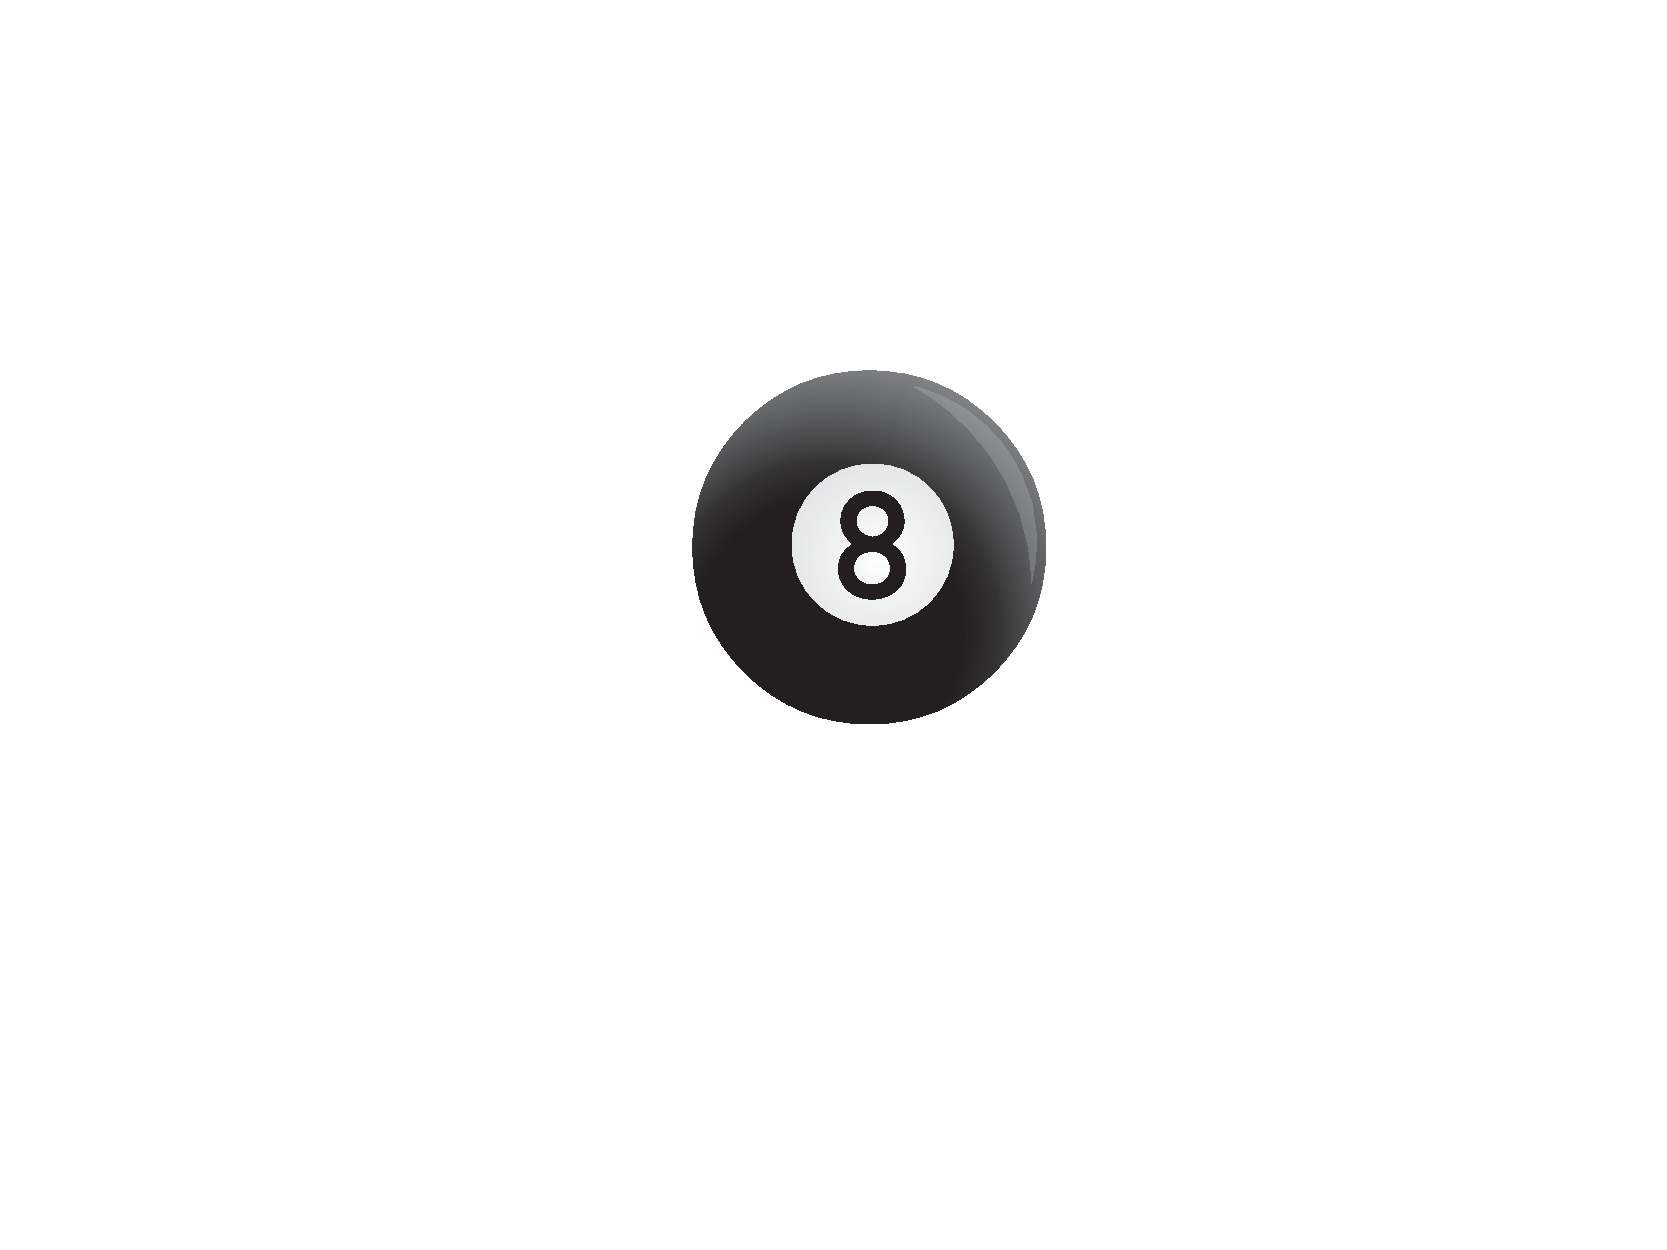
\includegraphics[width=.5\textwidth]{images/8ball}

    \par\vspace*{2\onelineskip}
	\par\par
    \par
    
    \large By Jesper Baekdahl and Simon Have
  }
  \vfill
  \vspace*{2\onelineskip}
  Supervisor: Zheng-Hua Tan
  Date: 28-5-2011
  \par\vspace*{2\onelineskip}
  \small
  Vision, Graphics and Interactive Systems\par
  Aalborg University
  \enlargethispage{2\onelineskip}
\end{titlingpage}


\begin{nopagebreak}
{\samepage
\begin{tabular}{r}
\parbox{\textwidth}{  \raisebox{11mm}{
\includegraphics[height=1.2cm]{aaulogo.pdf}}
\hfill \parbox{5.9cm}{\begin{tabular}{l}
{\textsf\small \textbf{Elektroniske Systemer}}\\
{\textsf\small \textbf{Institut 8}}\\
{\textsf\small Fredrik Bajers Vej 7 A1} \\
{\textsf\small 9220 Aalborg Ø} \\
{\textsf\small \url{http://es.aau.dk/}} \\
\end{tabular}}}
\\
\end{tabular}

\begin{tabular}{cc}
\parbox{7cm}{
\begin{description}

\item {\textbf Title:}

\projekt

\end{description}

\parbox{8cm}{

\begin{description}
\item {\textbf Project period:}\\
  	5. spring semester, 2009\\
  \hspace{4cm}
\item {\textbf Project group:}\\
  \gruppe\\
  \hspace{4cm}
\item {\textbf Group members:}\\
Jesper Birksø Bækdahl \\
Rolf Røgild Madsen \\
Simon Hartmann Have \\
  \hspace{2cm}
\item {\textbf Supervisor:}\\
Thomas Moeslund \\
\end{description}
}
\begin{description}
\item {\textbf Total number of copies:} 2
\item {\textbf Pages:} \pageref{LastPage}
\item {\textbf Addendum:} In appendix and enclosed with the report on a CD-ROM.
\item {\textbf Finished the} 2. June 2010
\end{description}
\vfill } &
\parbox{7cm}{
  \vspace{.15cm}
  \hfill
  \begin{tabular}{l}
  {\textbf Synopsis:}\bigskip \\
  \fbox{
    \parbox{6.5cm}{\bigskip
     {\vfill{\small This report describes the creation of a system with the capability of detecting and identifying pool table and balls using a standard webcam. A webcam is used to make the solution more attractive for consumers.

The game of pool has been analyzed along with the pool table and the balls. Especially colors of table and balls in different color spaces have been examined since this is what is used in the methods which contains detection and identification.

The solution is presented as a prototype system. The detection of table is done using the color information found in the analysis, and is successful. 

The positions of the balls are found using ball probability estimation. Detection works in all situations where balls are positioned apart, and in some situations where the balls are positioned in clusters.

The identification of the balls is done by using Euclidean distances between training data and detected data in RGB color space. The method works in some cases, but because of the webcam's inability to produce images with good color distribution it often fails.
     \bigskip}}
     }}
   \end{tabular}}
\end{tabular}}
\\ \\
%% eventuelt en footnote
\noindent{\footnotesize\emph{}}
\end{nopagebreak}


\section*{Preface}
This project should be understood by people who have a knowledge of computer vision and the different theories that are included in this field.

The software and videos used for this project are enclosed with the report on Aalborg University's project database.

\tableofcontents

\chapter{Introduction}
	\subsection{Project Background}
The inspiration for this project comes from the article "Development of an Automatic Pool Trainer"\cite{larsbopool} by LB Larsen et al which focused on making a pool trainer with only two different balls. The goal in this project is to extend the detection and matching part to be able to track a complete game of 8-ball pool with all 16 balls.
\\\\
Tracking pool games could be used for many different purposes. The pool trainer in \cite{larsbopool} could be extended to be able to train in environments that include more than two balls. This would provide for a more realistic training session when you have more than one choice of target. 

An automatic scoring system could be implemented by keeping track of which balls are still on the table.

The implementation used as an example in this project, is a pool history system, which makes the player able to se how the game has progressed by keeping track of the different states throughout the game. This will make the player able to improve and understand his own strengths and weaknesses.
\\\\
Previous attempts to track pool balls like \cite{supportBilliard} and \cite{ARPool}, only considered a 9-ball game where balls are separated and not positioned together in clusters. This project aims to detect and separate balls that are positioned in clusters, and to identify up to 16 balls, which is required for tracking a 8-ball game.
\\\\
It is a goal of this project to create a usable prototype, which could be installed by an end-user without having knowledge of computer vision. This requires the system to be adaptive towards variables like different lighting and ball colors. The user should be able to, place a camera above the pool table, turn on the system and after a short calibration process, track a pool game. The use of a standard webcam will make the solution inexpensive which is a key point when developing for personal use and entertainment.
\\\\
The solution will not include actual live tracking, but only the balls positions between shots. Further development of the solution could include this. As in \cite{larsbopool} the solution could also be expanded to use a projector to show ball positions, help lines for shooting balls in pockets and training environments. 

\subsection{Hypothesis}
How can we, with a standard inexpensive webcam, correctly detect a pool table and identify pool balls in mixed lighting?

\chapter{Analysis}
	To understand if the solution works it will be subjected to a test with origin in the requirement specification in section \ref{sec:reqspec}. The requirements, which will be tested, are listed here:

\begin{enumerate}
\setlength{\itemsep}{0mm}
	\item Detect position of table.
	\item Detect position of balls.
	\item Identify balls with high accuracy.
	\item Position and identification of balls should be obtained within one second
	\item Work with mixed light conditions and not only those stated in WPAB rules \ref{sec:rules}.
\end{enumerate}

The tests for the first four requirements will be done individually with the different lighting as described in section \ref{sec:testsetup}. The fifth requirement will be tested within the other requirements by altering the light.

\section{Test setup}
\label{sec:testsetup}
The test were conducted in the multimedia lab located in room A6-314 on Niels Jernes Vej 12 in Aalborg where image and video material for the solution to this project were made. 

%A second smaller test, to illustrate that the solution will work for different pool tables, is conducted in the DE-Klub which is a student bar located in A4-101 at Frederik Bajers Vej 7 in Aalborg. 
The pool table can be seen in figure \ref{fig:pooltableimg}. The videos used for the test can be found on the CD-Rom enclosed with this report.

\begin{figure}[H]
\begin{center}
\leavevmode
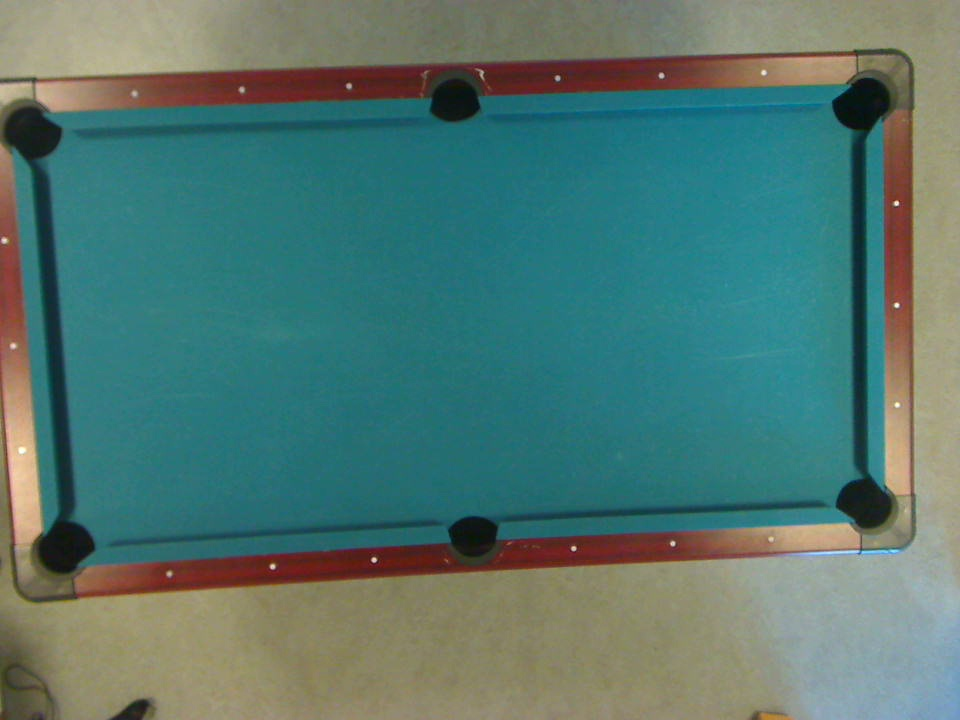
\includegraphics[width=0.4\textwidth]{images/test/light/input}
\end{center}
   \caption{The pool table used for testing.}
  \label{fig:pooltableimg}
\end{figure} 

The tests were made in two light conditions: normal and mixed. These conditions can be seen in figure \ref{fig:difflightcon}.

\begin{figure}[H]
  \centering
  \subfloat[Normal illumination]{\label{fig:gull}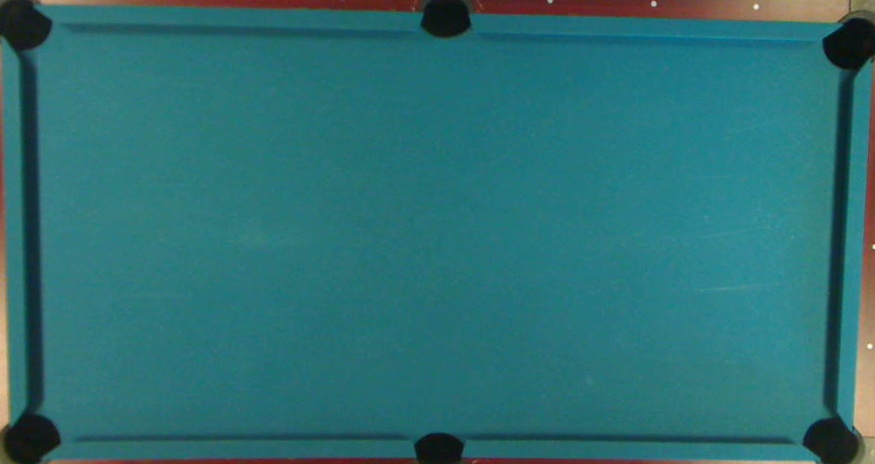
\includegraphics[width=0.48\textwidth]{images/test/light/detectedtable}}
  \quad           
  \subfloat[Mixed illumination]{\label{fig:tiger}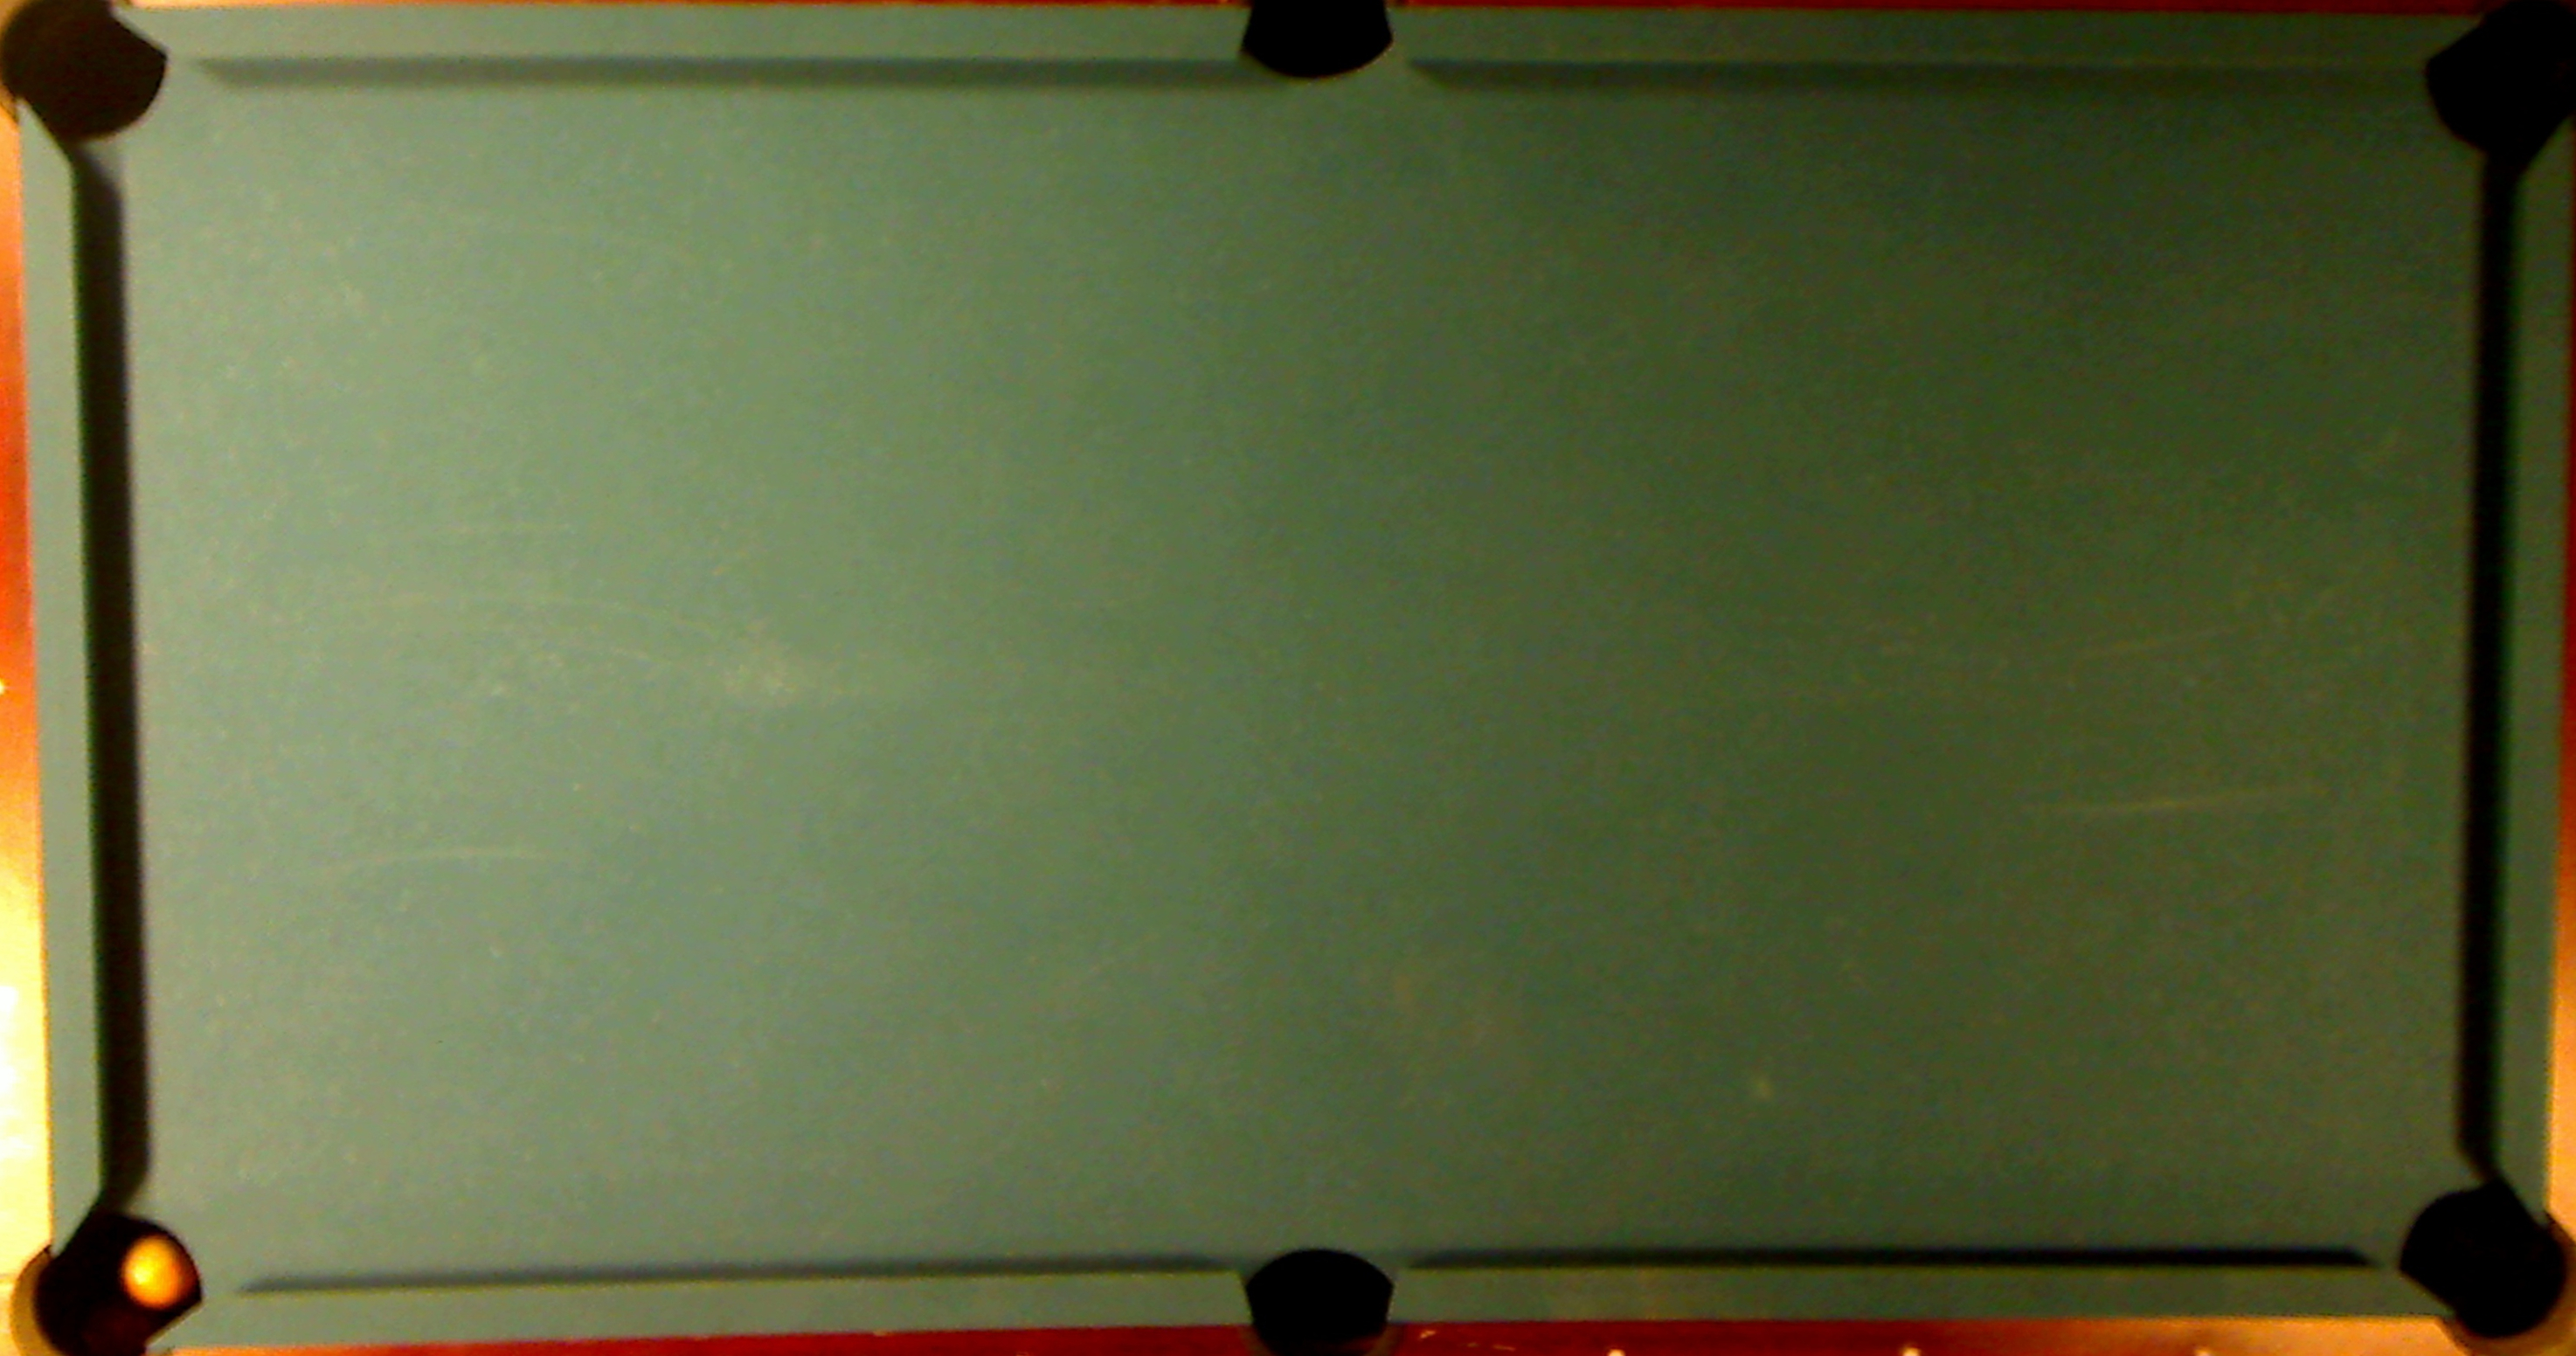
\includegraphics[width=0.48\textwidth]{images/test/mixed/detectedtable}}
   \caption{Table cloth in the two different light conditions.}
  \label{fig:difflightcon}
\end{figure}


\section{1) Detect position of table}

This was tested numerous times and if the position of the table is within the view of the camera the table will be found in both light conditions.

\section{2) Detect position of balls}
The precision of the ball positions is important, since the identification rests on having the correct positions. To test the detection, the balls have been positioned in different scenarios to test for different kinds of weaknesses in the detector. The following scenarios has been tested:
\begin{enumerate}
	\item Balls laying apart.
	\item Balls clustered by color
	\item Balls laying in start position as described in section \ref{sec:rules}.
\end{enumerate}
In some of the tests, two results have been recorded. One representing the best case scenario and one representing the worst case scenario. This is done to illustrate the differences observed during the test.

\subsection{Balls laying apart}
The least difficult test for the detection of balls is where the balls are laying apart. The result of the test with normal light can be seen in figure \ref{fig:apartnormal} and for the mixed light in figure \ref{fig:apartmixed}.

\begin{figure}[htpb]
  \centering
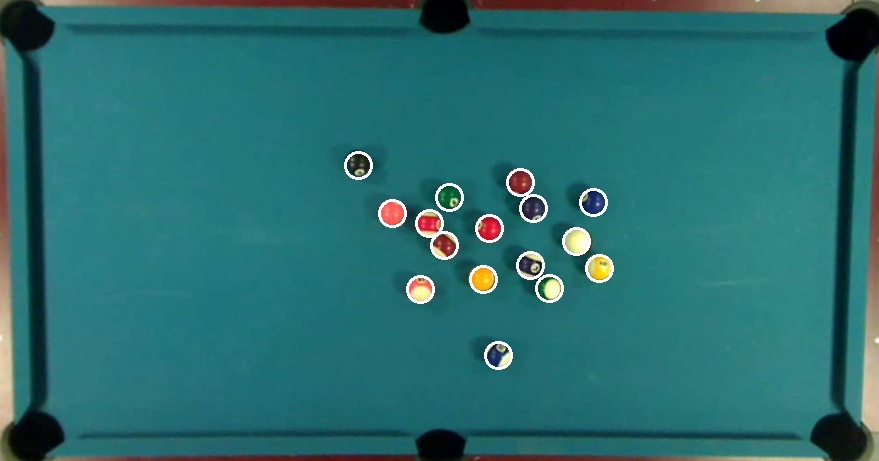
\includegraphics[width=0.5\textwidth]{images/test/light1/laying-apart}
   \caption{Balls laying apart - normal light.}
  \label{fig:apartnormal}
\end{figure}

\begin{figure}[htpb]
  \centering
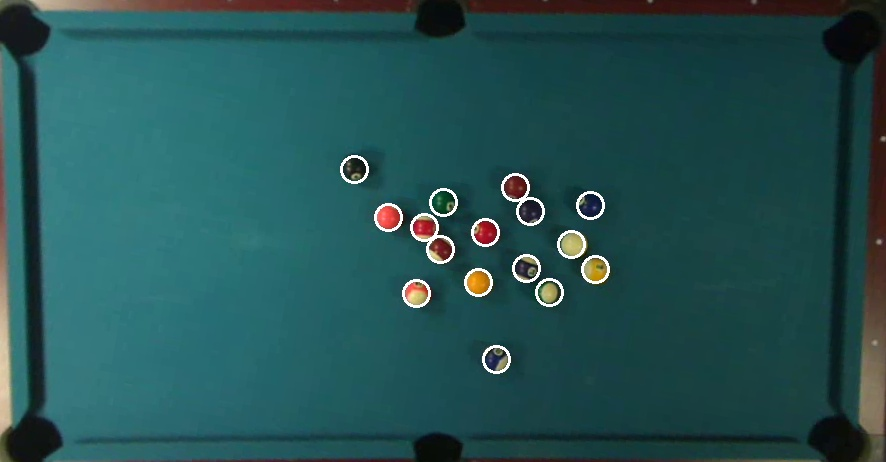
\includegraphics[width=0.5\textwidth]{images/test/mixed1/laying-apart}
   \caption{Balls laying apart - mixed light.}
  \label{fig:apartmixed}
\end{figure}

There is no significant change in the behavior of the system between the mixed, and the normal lighting. The balls are detected correctly in both the left and the right side of the table. This shows that the detection is adaptive towards change in lighting across the table in an uncluttered ball arrangement.

\subsection{Balls clustered by color}
As mentioned in section \ref{sec:balls-locate}, the ball detection works by finding areas that minimizes the color variance. To test for weaknesses in this method, the scenario seen in figures \ref{fig:clustersnormal} and \ref{fig:clustersmixed} is tested.
\begin{figure}[htpb]
  \centering
  \subfloat[Black ball low precision]{\label{fig:gull}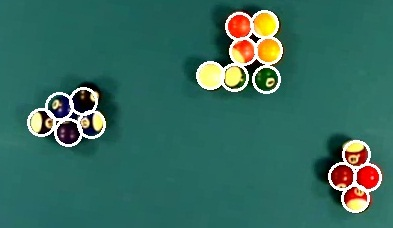
\includegraphics[width=0.4\textwidth]{images/test/light1/clusters-1}}
  \quad
   \subfloat[Two balls detected wrong]{\label{fig:tiger}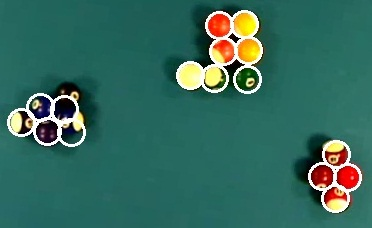
\includegraphics[width=0.4\textwidth]{images/test/light1/clusters-2}}
	\quad
   \caption{Balls in clusters - normal light.}
  \label{fig:clustersnormal}
\end{figure}

\begin{figure}[htpb]
  \centering
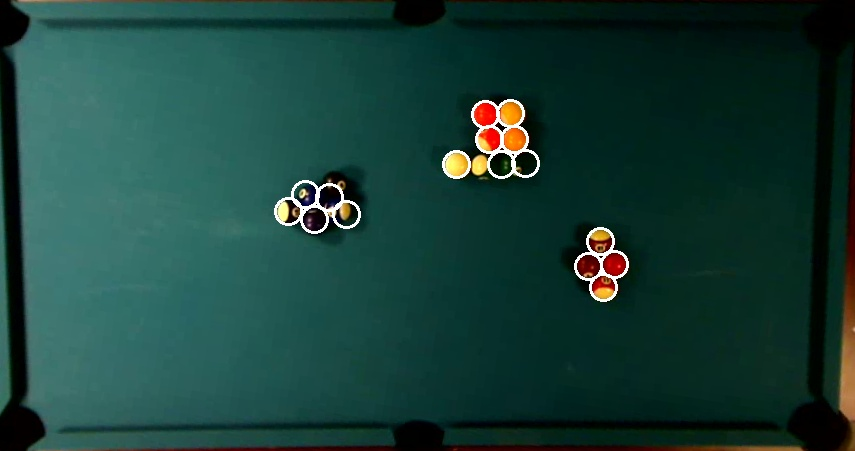
\includegraphics[width=0.5\textwidth]{images/test/mixed1/clusters-2}
   \caption{Balls in clusters - mixed light. Several detection problems.}
  \label{fig:clustersmixed}
\end{figure}
The balls are not correctly detected in this scenario. The problem is most significant in the left cluster that consists of the dark colored balls: purple, blue and black. The problem worsens when the image is darker in figure \ref{fig:clustersmixed}. The detection of the red colored balls does however not result in any errors or positional problems. 


\subsection{Balls laying in start position}
The balls are placed in the start position with all balls except the cue ball clustered. This is the most difficult condition to test positions of the pool balls. The test was done while the balls were laying still and the result of the test with normal light can be seen in figure \ref{fig:poolposstart} and for the mixed light in figure \ref{fig:poolposstart2}.

\begin{figure}[htpb]
  \centering
   \subfloat[Correct detection]{\label{fig:poolposstart-good}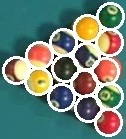
\includegraphics[width=0.2\textwidth]{images/test/light1/start-normal-1}}
\quad
   \subfloat[Incorrect detection]{\label{fig:poolposstart-bad}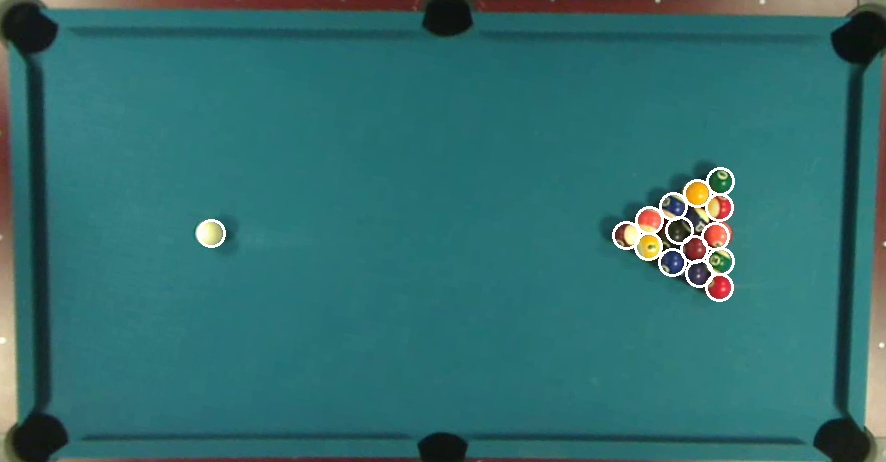
\includegraphics[width=0.2\textwidth]{images/test/light1/start-normal-2}}
   \caption{Balls in start position - normal light.}
  \label{fig:poolposstart}
\end{figure}

\begin{figure}[htpb]
  \centering
  \subfloat[Correct detection]{\label{fig:gull}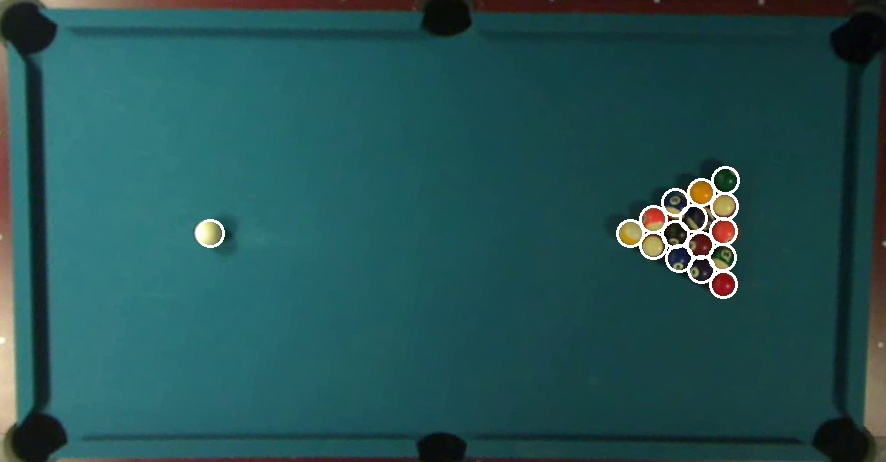
\includegraphics[width=0.2\textwidth]{images/test/mixed1/start-mixed-1}}
\quad
   \subfloat[Incorrect detection]{\label{fig:tiger}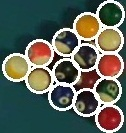
\includegraphics[width=0.2\textwidth]{images/test/mixed1/start-mixed-2}}
\quad
   \caption{Balls in start position - mixed light.}
  \label{fig:poolposstart2}
\end{figure}

The system performs almost equally in the light environment seen in figure \ref{fig:poolposstart} as in mixed lighting in figure \ref{fig:poolposstart2}. For the system to find all positions in this situation, it is important that the positions of the first detected balls are correct, because their positions will affect the rest of the detection as mentioned in section \ref{sec:balls-locate}. Problems arise in a situation like the one seen in figure \ref{fig:poolposstart-bad}. The black and orange balls have been inaccurately detected, and the consequence is that there is insufficient room to detect the striped purple 14.


\section{Identify balls with high accuracy}
The identification of the balls is done by first calibrating the system and then testing the identification with the balls facing in two different scenarios:

\begin{enumerate}
\setlength{\itemsep}{0mm}
	\item \textbf{Minimum} white area visible
	\item \textbf{Maximum} white area visible
\end{enumerate}
This is done to test the borderline cases for when a ball is considered solid, striped or white.

\subsection{Pool balls laying with minimum white facing up}
This scenario will test if the identifier has problems that causes striped balls to be identified as solid balls.
The result of the test with normal light can be seen in figure \ref{fig:minnormal} and for the mixed light in figure \ref{fig:minmixed}.
\begin{figure}[htpb]
  \centering
  \subfloat[Input image]{\label{fig:gull}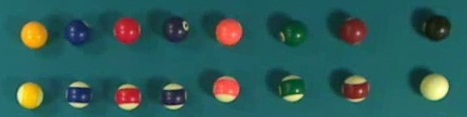
\includegraphics[width=0.5\textwidth]{images/test/light1/min-white-input}}
  \quad
   \subfloat[Found balls]{\label{fig:tiger}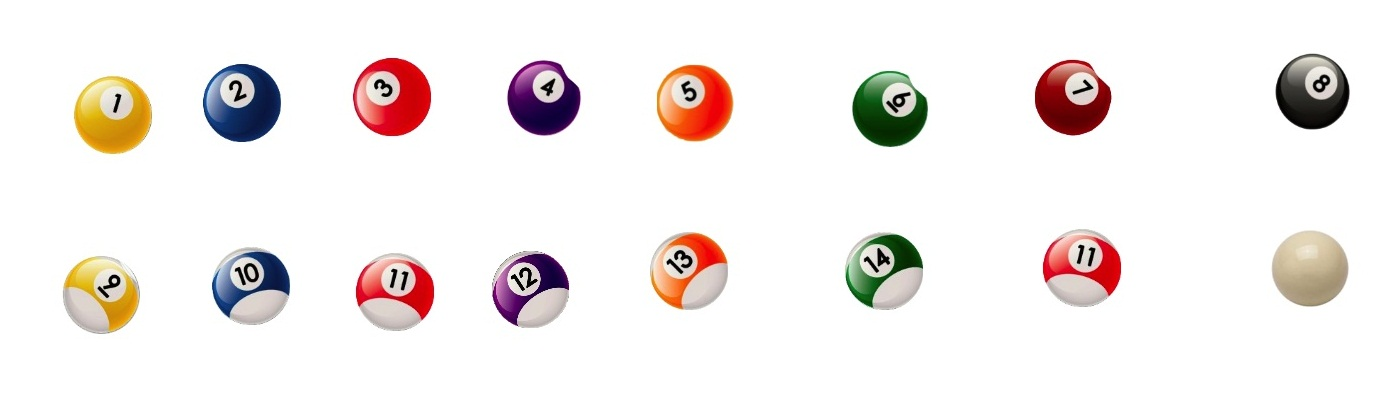
\includegraphics[width=0.5\textwidth]{images/test/light1/min-white-output}}
	\quad
   \caption{Balls having minimum white area visible - normal light.}
  \label{fig:minnormal}
\end{figure}

\begin{figure}[htpb]
  \centering
  \subfloat[Input image]{\label{fig:gull}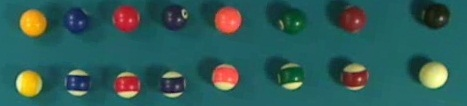
\includegraphics[width=0.5\textwidth]{images/test/mixed1/min-white-input}}
  \quad
  \subfloat[Found balls]{\label{fig:tiger}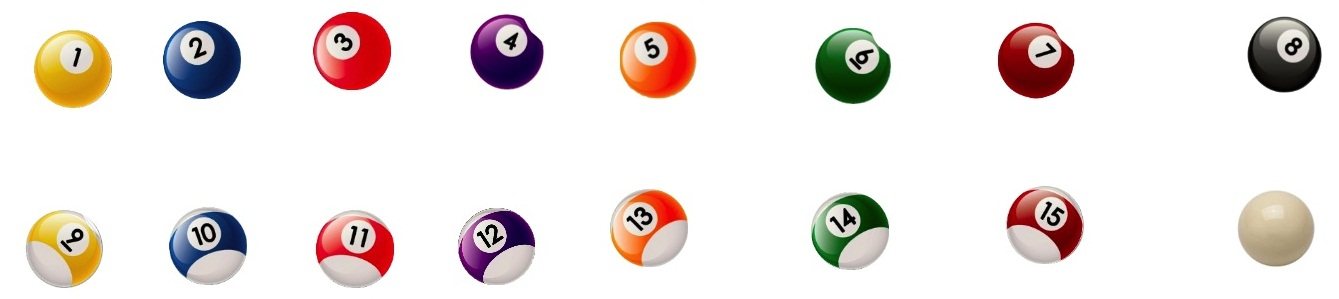
\includegraphics[width=0.5\textwidth]{images/test/mixed1/min-white-output}}
  \quad
   \caption{Balls having minimum white area visible - mixed light.}
  \label{fig:minmixed}
\end{figure}
All balls on both mixed and normal lighting are correctly identified, except for striped brown 15 which has been classified as red striped 11. This occurs because of the colors begin close. None of the striped balls are misclassified as solids, independent of lighting conditions.

\subsection{Pool balls laying with maximum white facing up}
This test will illustrate if the ratio of white pixels is defined well enough to identify if the ball is solid or striped. Also the detection of correct colors will be tested. The result of the test with normal light can be seen in figure \ref{fig:maxnormal} and for the mixed light in figure \ref{fig:maxmixed}.

\begin{figure}[htpb]
  \centering
  \subfloat[Input image]{\label{fig:gull}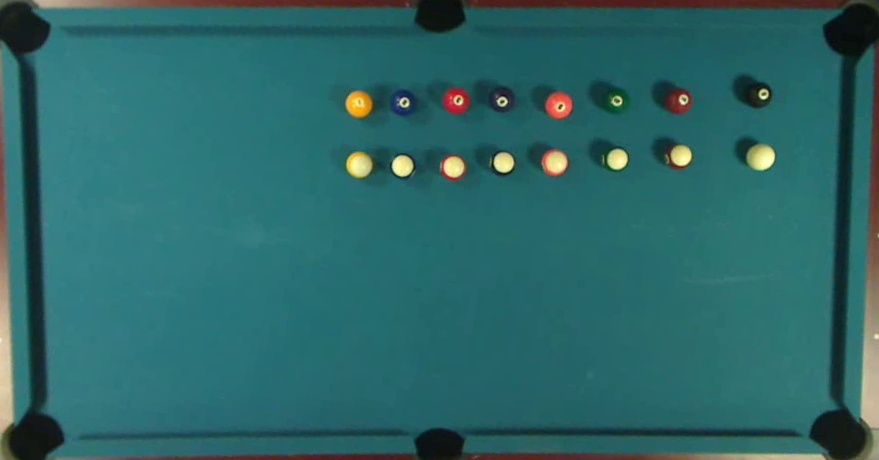
\includegraphics[width=0.5\textwidth]{images/test/light1/max-white-input}}
  \quad
   \subfloat[Found balls]{\label{fig:tiger}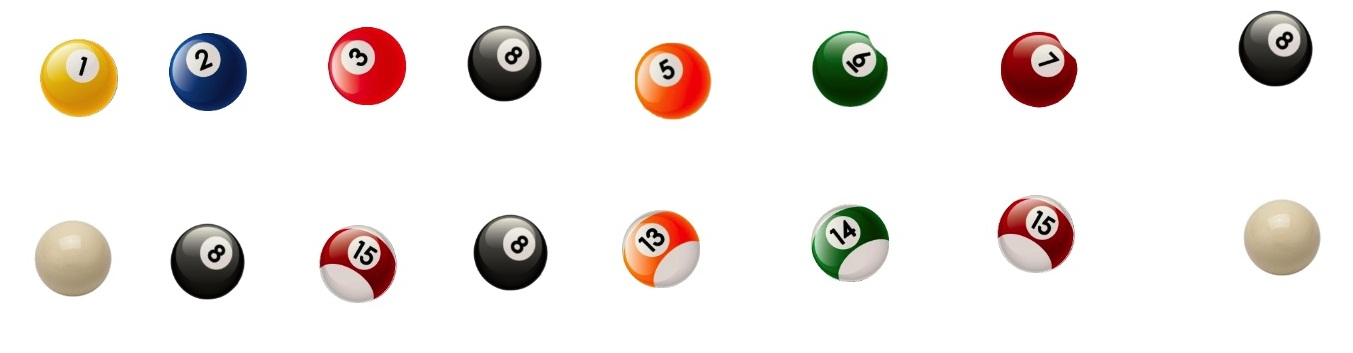
\includegraphics[width=0.5\textwidth]{images/test/light1/max-white-output}}
	\quad
   \caption{Balls having maximum white area visible - normal light.}
  \label{fig:maxnormal}
\end{figure}

\begin{figure}[htpb]
  \centering
  \subfloat[Input image]{\label{fig:gull}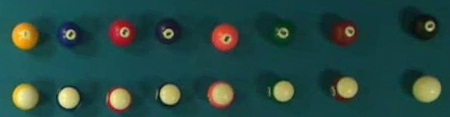
\includegraphics[width=0.5\textwidth]{images/test/mixed1/max-white-input}}
  \quad
  \subfloat[Found balls]{\label{fig:tiger}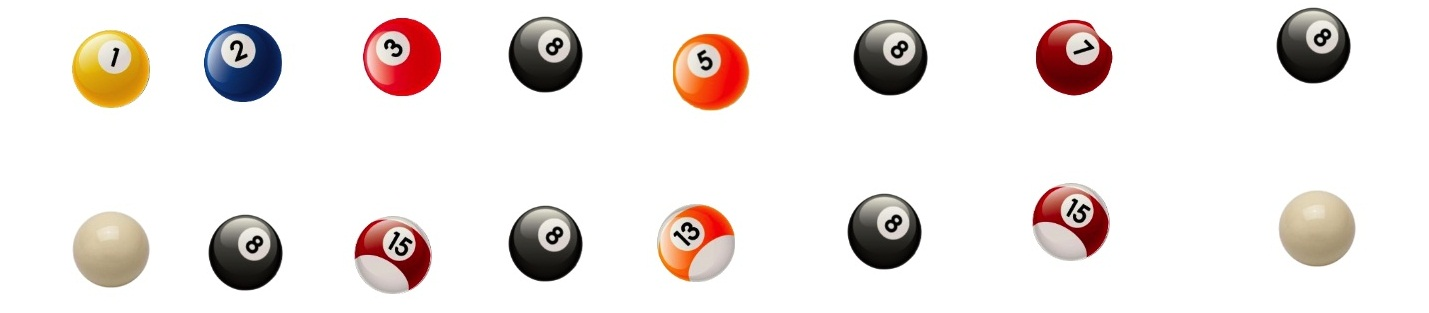
\includegraphics[width=0.5\textwidth]{images/test/mixed1/max-white-output}}
  \quad
   \caption{Balls having maximum white area visible - mixed light.}
  \label{fig:maxmixed}
\end{figure}
The identification fails in both normal and mixed light. Identification of the striped balls in this scenario is problematic due to the small amount of color available. Most of the striped balls are however, identified as being striped in spite of the small amount of color. In the mixed light environment, several of the balls are identified as being the black 8-ball which is caused by the identifier being sensitive to the change in lighting.

\subsection{Position and identification of balls should be obtained within one second}
The system speed was tested with different sizes of video and image input from the used webcam. It will find the position and identify the balls within one second. This test was done on a Core-Duo L2400 running at 1.67 Ghz. 

	\label{sec:analysis}
	
	\section{About Pool}

		\subsection{Pool table specifications and rules}
			\label{sec:rules}
			This project will focus on pool tables (pocket billiards). There are many different types of pool such as 8-ball, 9-ball and 14-1. The types differentiate some, but the table and the rest of the equipment is the same. 

 The international pool regulations concerning table size, cloth colour, ball size and etc. are regulated by "World Pool-Billiard Association". These specifications will be understood in order to know what size of table, ball etc. that has to be looked for while doing the image processing.


In \ref{fig:partspool} a standart pool table is seen from top view. Different indications of pockets etc. are marked.

\begin{figure}[H]
\begin{center}
\leavevmode
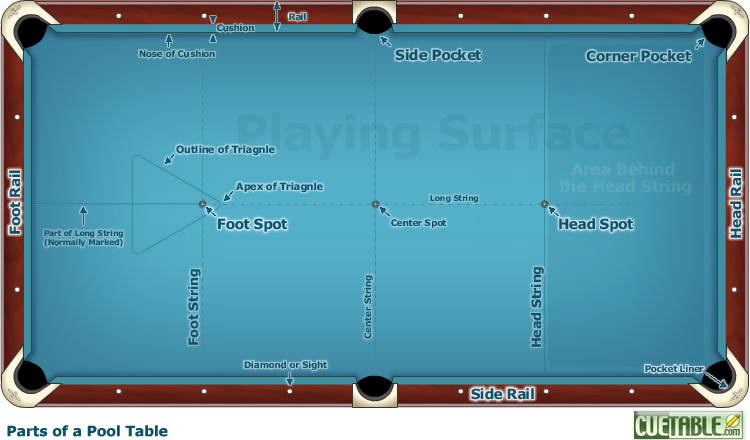
\includegraphics[width=0.9\textwidth]{images/pooltablespecs.jpg}
\end{center}
\caption{Parts of pool table. From cuetable.com}
\label{fig:partspool}
\end{figure}

The, for this project, important regulations are listed here:
\begin{itemize}
	\item \textbf{Playing surface size:}\\
		Must be rectangular and symmetrical.\\
		9. foot table: 2.54 x 1.27 m.\\
		8. foot table: 2.34 x 1.68 m.\\
	\item \textbf{Rail size:}\\
		Must be between 10.16 and 19.05 cm including the rubber cushions.\\
	\item \textbf{Diamonds (sights):}\\
		18 diamonds (sights) (or 17 and a name plate) must be attached flush on the rail cap with:\\
		9. foot table: 31.75 cm from diamond to diamond.\\
		8. foot table: 29.20 cm from diamond to diamond.\\
		The center of each diamond should be located 93.5 mm from the nose of the cushion.\\
		The diamonds may be round or diamond-shaped.\\
	\item \textbf{Cloth:}\\
		Only the colors of yellow-green, blue-green or electric blue are acceptable for WPA competition. \\
	\item \textbf{Ball size:}\\
		All balls should be 5.715 cm in diameter.\\
		A complete set of balls consist of:\\
		Que ball: White\\
		Solid colors:\\
		\hspace*{10 mm}	1:Yellow, 2:Blue, 3:Red, 4:Purple, 5:Orange, 6:Green, 7: Maroon, 8:Black.\\
		Balls with centered band:\\
		\hspace*{10 mm}	9:Yellow, 10:Blue, 11:Red, 12:Purple, 13:Orange, 14:Green, 15:Maroon\\


	

\end{itemize}
	
		\subsection{Color analysis of table and balls}
			\label{sec:analysisballstable}
			To detect the pool table and balls it is important to understand how they appear in different color spaces. In this section the colors of the table and the pool balls are measured for further analysis.

\section{The Table}
As written in the rules in section \ref{sec:rules}, the table cloth color has to be yellow-green, blue-green or electric blue. The cloth color is a constant color, but dependent on the lighting, the cloth color could have some variance.

Three different images of the pool table and one image with the cloth cut out are analyzed first in HSB color space and then i RGB space. These analysis will be used in the solution chapter.

\begin{figure}[H]
\begin{center}
\leavevmode
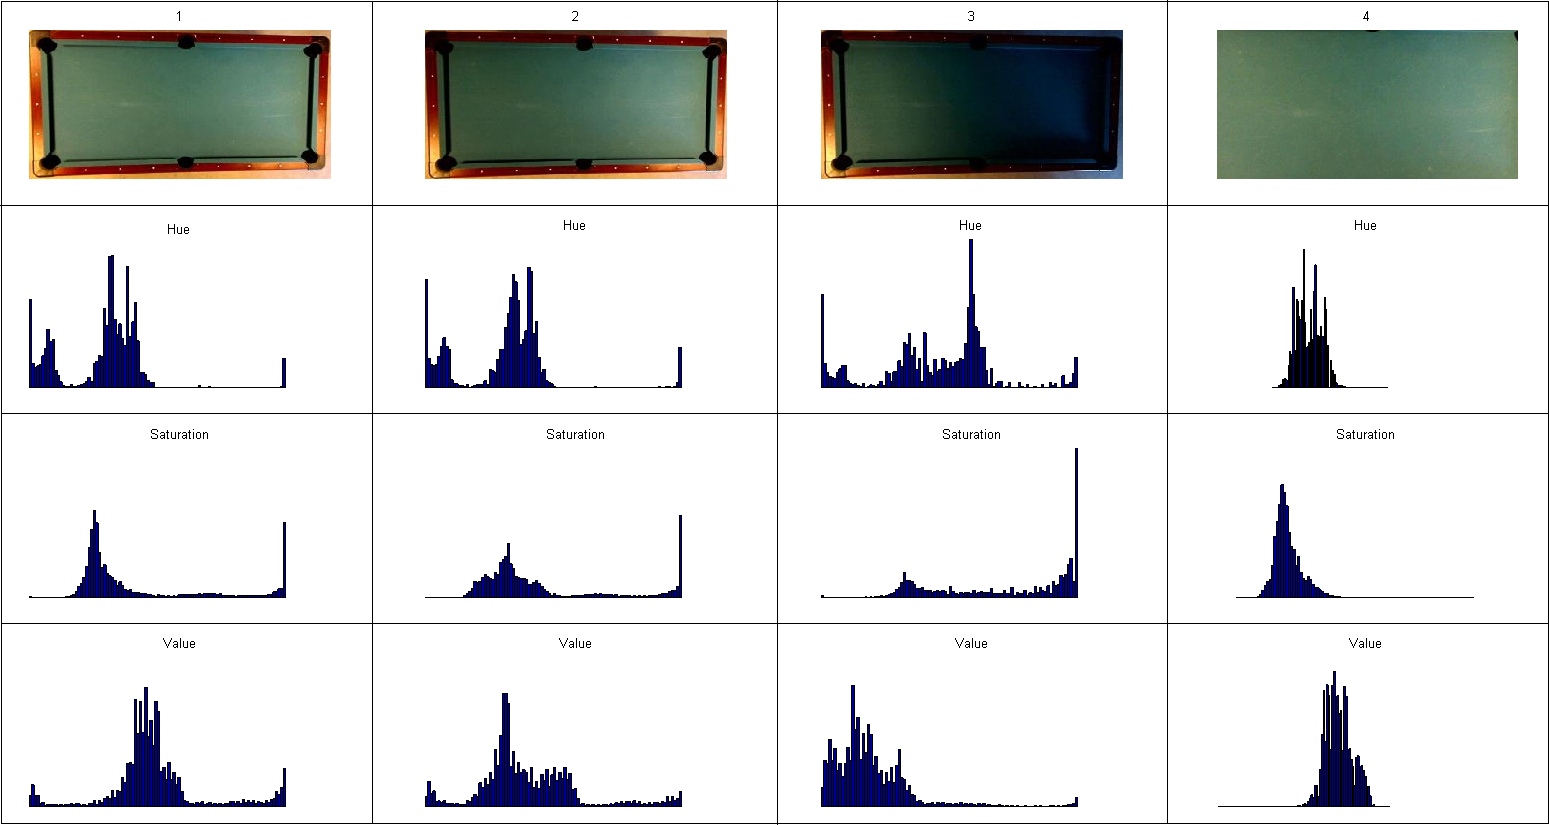
\includegraphics[width=0.6\textwidth]{images/hsv_hist_table}
\end{center}
\caption{HSB Images 1, 2 and 3 are the table in different light where 4 is the cutout of the cloth from image 1. All axis are aligned.}
\label{fig:tablehsv}
\end{figure} 

From the HSB color space figure \ref{fig:tablehsv} it is clear that the cloth should be somewhat easily detected using hue for the fist two images. The separation of rail and cloth is not as significant in the third image. This is because of the different illumination, which is very dark. In section \ref{sec:camera} different camera settings and illuminations are discussed which indicates that the third image is less illuminated than should be for this project.
\begin{figure}[H]
\begin{center}
\leavevmode
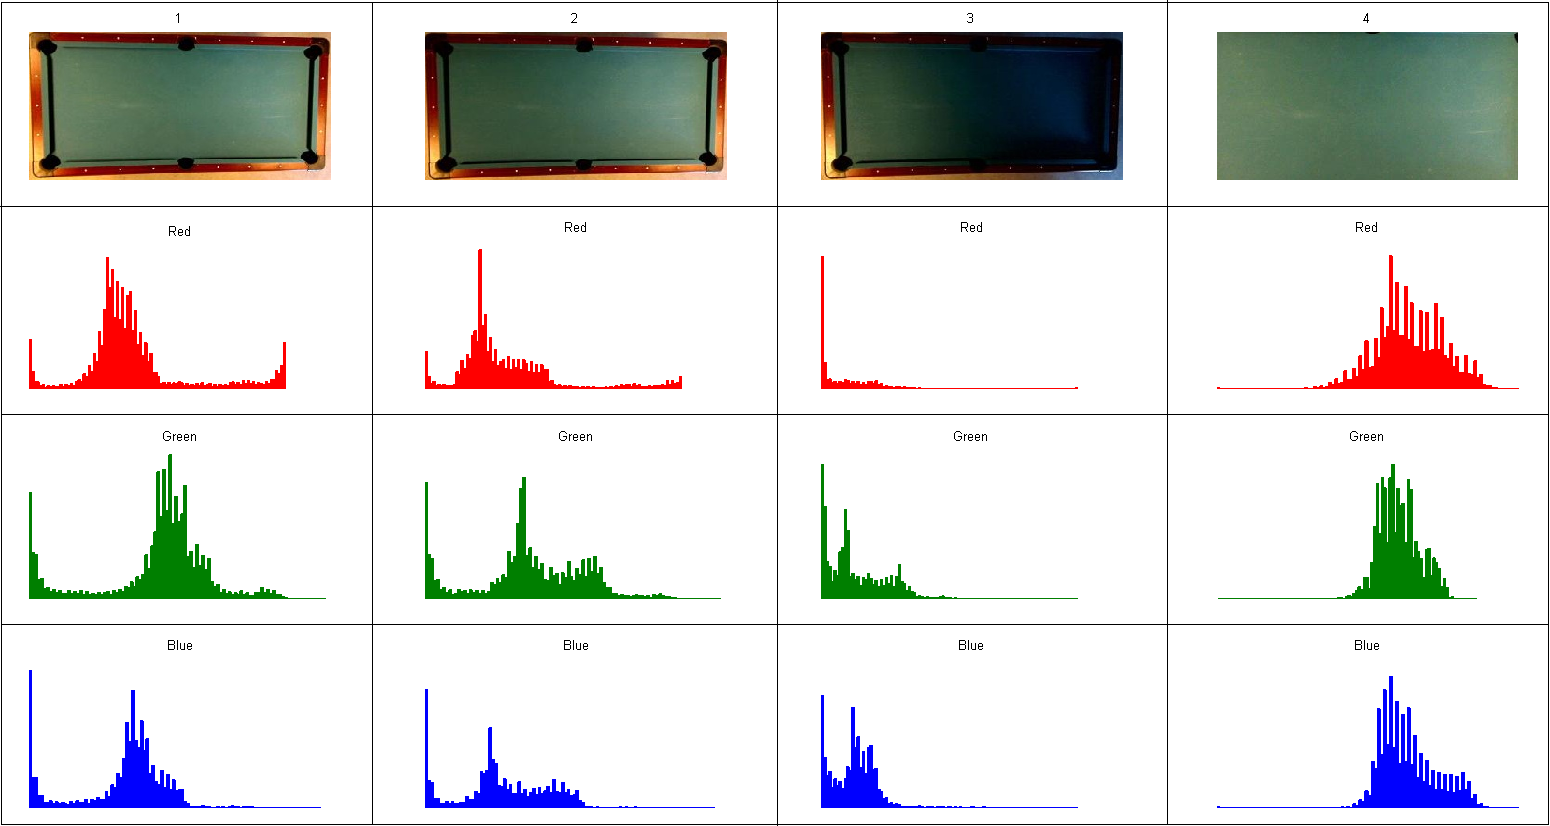
\includegraphics[width=0.6\textwidth]{images/rgb_hist_table}
\end{center}
\caption{RGB Images 1, 2 and 3 are the table in different light where 4 is the cutout of the cloth from image 1. All axis are aligned.}
\label{fig:tablergb}
\end{figure}
When looking at the RGB color space in figure \ref{fig:tablergb} the identification of the cloth becomes more difficult. 
As presumed, it is easier to identify the cloth in the hue-space in figure \ref{fig:tablehsv} than in either of the RGB color space components in figure \ref{fig:tablergb}. This is because of the hue ability to be, in theory, brightness invariant.

\section{The Balls}
\label{sec:analballs}
The success of the system depends on the identifiers ability to separate the pool balls from each other. To analyze the separability, histograms of all the different solid colored balls have been computed. This is done in hue-saturation space, to see if it is possible to be independent of brightness. If the system is independent of brightness, it will be more resistant towards changes in illumination. The histograms are arranged pairwise together in the same figure, based on color similarity, to visualize how the colors can be separated.

\begin{figure}[H]
\centering
\subfloat
{
	
\includegraphics[width=0.4\textwidth]{images/ballhist/0}
}
\subfloat
{
	
\includegraphics[width=0.4\textwidth]{images/ballhist/8}
}
\caption{Color histogram of cue-ball and 8-ball}
\label{fig:ballhist-cue-8}
\end{figure}
Figure \ref{fig:ballhist-cue-8} shows the histograms of the cue-ball and the 8-ball. The cue-ball distribution is isolated in a low-saturation area, having a yellow hue around 50. The saturation of the other balls is generally above the white saturation, making it possible to identify white pixels by setting a saturation threshold.

The hue-saturation distribution of the 8-ball is scattered all over the range. The reason for this, is that black is undefined in hue-saturation space. Black will have to be detected by the brightness value, which is significantly lower than other balls. \fxnote{VALUE HISTOGRAM HERE.}

\begin{figure}[H]
\centering
\subfloat
{
	
\includegraphics[width=0.4\textwidth]{images/ballhist/3}
}
\subfloat
{
	
\includegraphics[width=0.4\textwidth]{images/ballhist/5}
}

\subfloat
{
	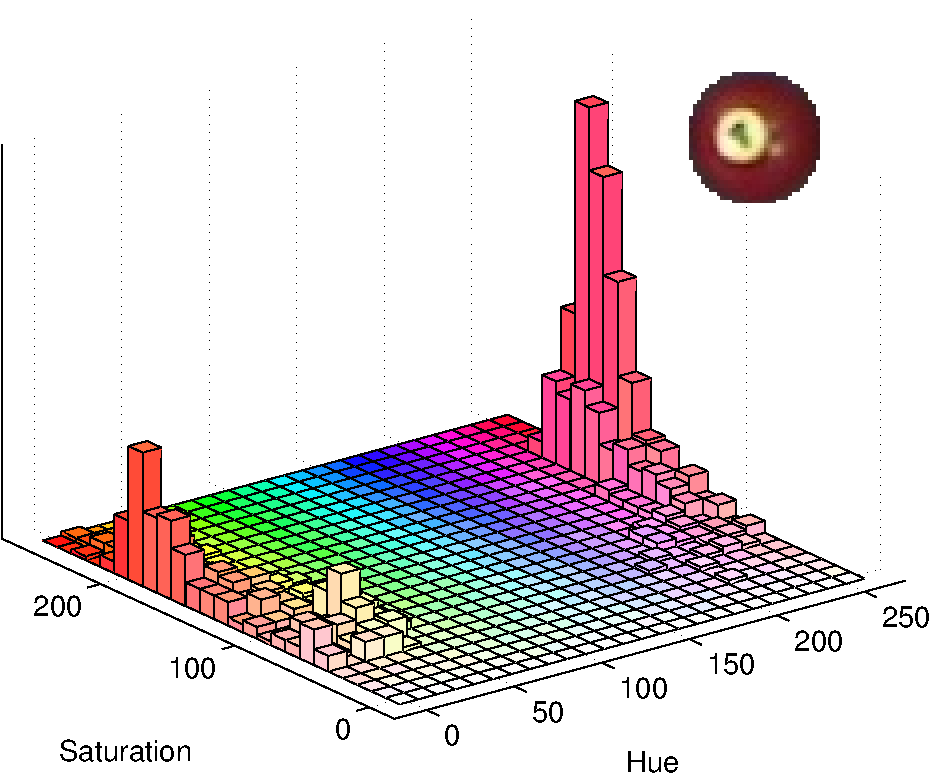
\includegraphics[width=0.4\textwidth]{images/ballhist/7}
}

\caption{Color histogram of balls: 3, 5 and 7}
\label{fig:ballhist-3-7}
\end{figure} 
Figure \ref{fig:ballhist-3-7} shows a situation where the balls are going to be difficult to separate. Depending on the lighting and camera settings, the color of 3, 5 and 7 have almost the same hue, and are only separable in saturation.

The histograms in figure \ref{fig:ballhist-3-7} also show one of the weaknesses of using HSB colorspace which is the that hue is defined an angular value that wraps between minimum and maximum. The consequence of this is that the 3 balls which has red as their dominant hue have one distribution near minimum hue and one near maximum.
\begin{figure}[H]
\centering
\subfloat
{
	
\includegraphics[width=0.4\textwidth]{images/ballhist/2}
}
\subfloat
{
	
\includegraphics[width=0.4\textwidth]{images/ballhist/4}
}
\caption{Color histogram of balls: 2 and 4}
\label{fig:ballhist-2-4}
\end{figure}
Figure \ref{fig:ballhist-2-4} shows that the blue and purple balls are also challenging to separate.

\begin{figure}[H]
\centering
\subfloat
{
	
\includegraphics[width=0.4\textwidth]{images/ballhist/1}
}
\subfloat
{
	
\includegraphics[width=0.4\textwidth]{images/ballhist/6}
}
\caption{Color histogram of balls: 1 and 6}
\label{fig:ballhist-1-6}
\end{figure} 
Figure \ref{fig:ballhist-1-6} shows the two balls which do not have close neighbors. The green ball does however contain colors that are very similar to the color of the table cloth, making it harder to separate from the background than the rest.



\subsection{Ball Color Composition}
To be able to detect whether or not a ball is solid or striped it is important to know how big a portion of a ball is white. The images used can be seen in figure \ref{fig:ballscompo} which is based on the balls used in this project.

\begin{figure}[htpb]
\centering
\subfloat[Solid ball with number turned up.]
{
	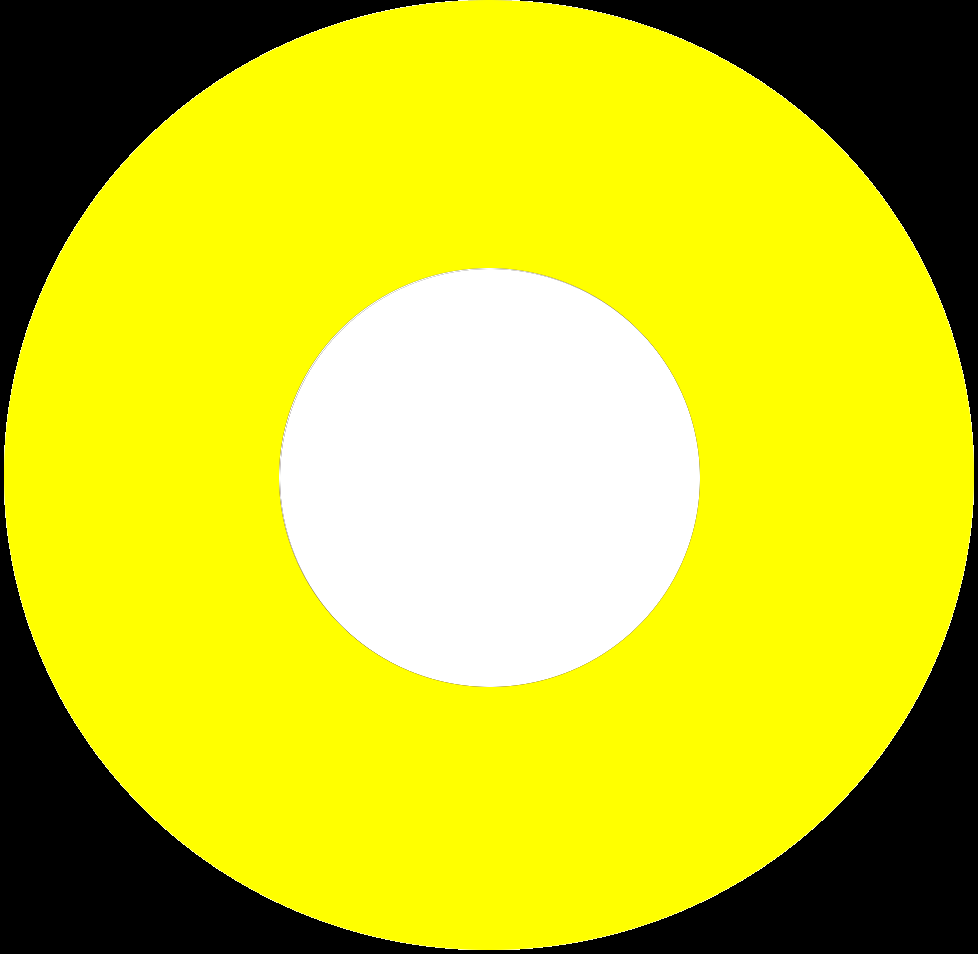
\includegraphics[width=0.2\textwidth]{images/fy.png}
}
\quad
\subfloat[Striped ball with minimum white.]
{
	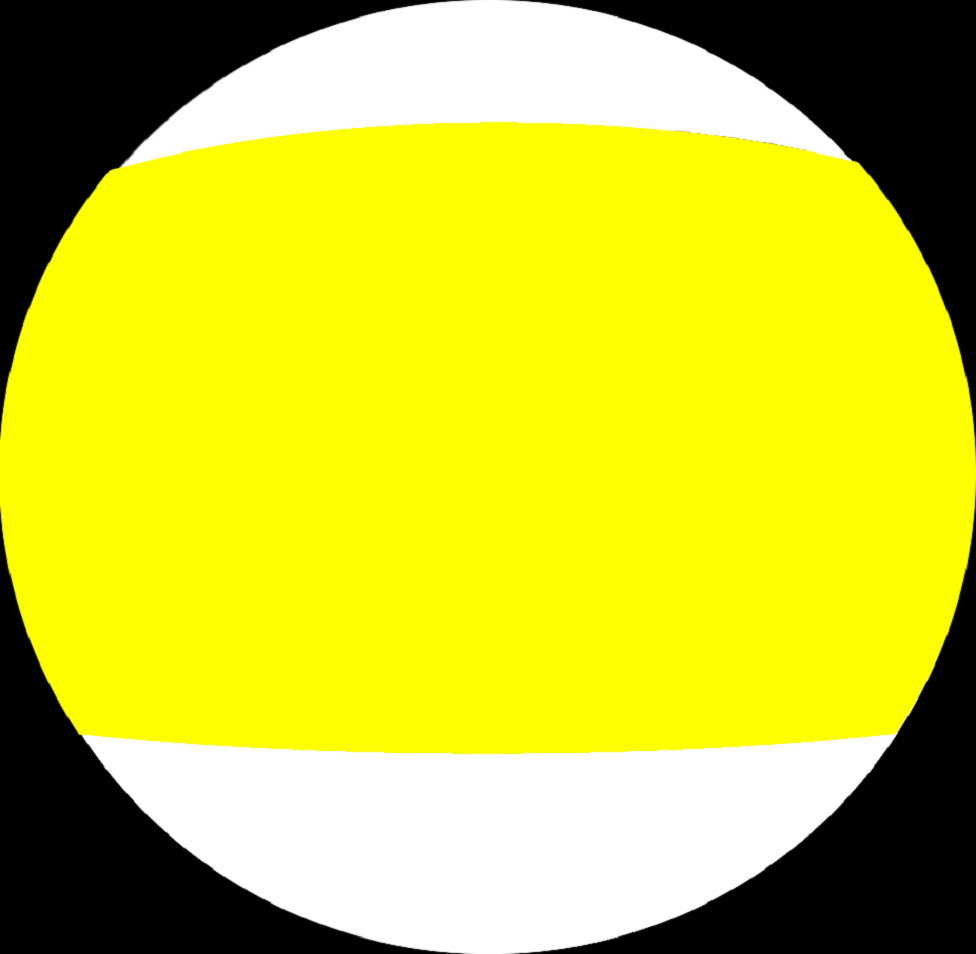
\includegraphics[width=0.2\textwidth]{images/fymax.png}
}
\quad
\subfloat[Striped ball with maximum white.]
{
	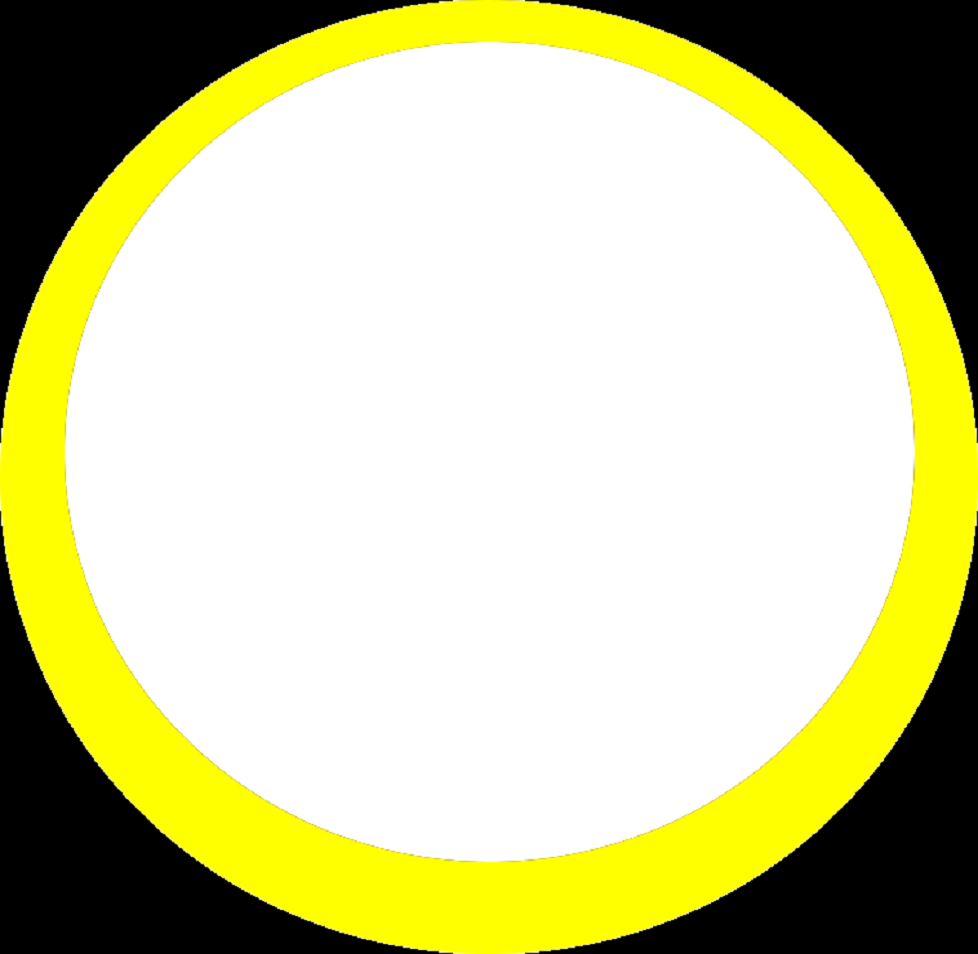
\includegraphics[width=0.2	\textwidth]{images/fymin.png}
}

\caption{Ball color compositions.}
\label{fig:ballscompo}
\end{figure}

In table \ref{fig:ballscompotable} the percentage of white pixels can be seen.

\begin{table}[htpb]
\centering
\begin{tabular}{|c|c|c|c|}
	\hline Figure & a) & b) & c) \\ 
	\hline Color & 583217 & 548839 & 175858 \\ 
	\hline White & 137359 & 173401 & 542900 \\ 
	\hline Percentage & 19.0\% & 24.0\% & 75.5\% \\ 
	\hline
\end{tabular}
\caption{Table with ball color composition.}
\label{fig:ballscompotable}
\end{table}


		\subsection{Pool terminology}
			\label{sec:terminology}
			\input{analysis/terminology}
	
		\subsection{Pool situations}
			\label{sec:situations}
			\input{analysis/situations}
	
		
	\section{Other work}
		\label{sec:otherwork}
		\input{analysis/otherwork}
					
	\section{Requirements specification}
		\label{sec:reqspec}
		The goal for the project is to do the following:

\begin{itemize}
\setlength{\itemsep}{0mm}
	\item Detect position of table.
	\item Detect position of balls.
	\item Identify balls with high accuracy.
	\item Position and identification of balls should be obtained within one second
	\item Work with mixed light conditions and not only those stated in WPAB rules\ref{sec:rules}.
	\item Be made into a working prototype.
%	\item Be easily used by players. %Lars Bo Warning!
\end{itemize}

The completed system is not required to:

\begin{itemize}
\setlength{\itemsep}{0mm}
	\item Calibrate camera parameters and undistort image.
	\item Track balls when they are moving.
	\item Act as a referee and make the players obey the rules.
	\item Work with very difficult light conditions.
\end{itemize}

For the system to work certain requirements must be set:
\begin{itemize}
\setlength{\itemsep}{0mm}
	\item The full table must take up 75\% of the image and  be viewable with no parts occluded.
	\item The exposure and focus of the camera must be optimal and oversaturation should not occur.
	\item Ball coloring and cloth coloring must follow WPAB regulations as described in \ref{sec:rules}.
\end{itemize}

\chapter{Solution}
	\label{solution}
	To understand if the solution works it will be subjected to a test with origin in the requirement specification in section \ref{sec:reqspec}. The requirements, which will be tested, are listed here:

\begin{enumerate}
\setlength{\itemsep}{0mm}
	\item Detect position of table.
	\item Detect position of balls.
	\item Identify balls with high accuracy.
	\item Position and identification of balls should be obtained within one second
	\item Work with mixed light conditions and not only those stated in WPAB rules \ref{sec:rules}.
\end{enumerate}

The tests for the first four requirements will be done individually with the different lighting as described in section \ref{sec:testsetup}. The fifth requirement will be tested within the other requirements by altering the light.

\section{Test setup}
\label{sec:testsetup}
The test were conducted in the multimedia lab located in room A6-314 on Niels Jernes Vej 12 in Aalborg where image and video material for the solution to this project were made. 

%A second smaller test, to illustrate that the solution will work for different pool tables, is conducted in the DE-Klub which is a student bar located in A4-101 at Frederik Bajers Vej 7 in Aalborg. 
The pool table can be seen in figure \ref{fig:pooltableimg}. The videos used for the test can be found on the CD-Rom enclosed with this report.

\begin{figure}[H]
\begin{center}
\leavevmode
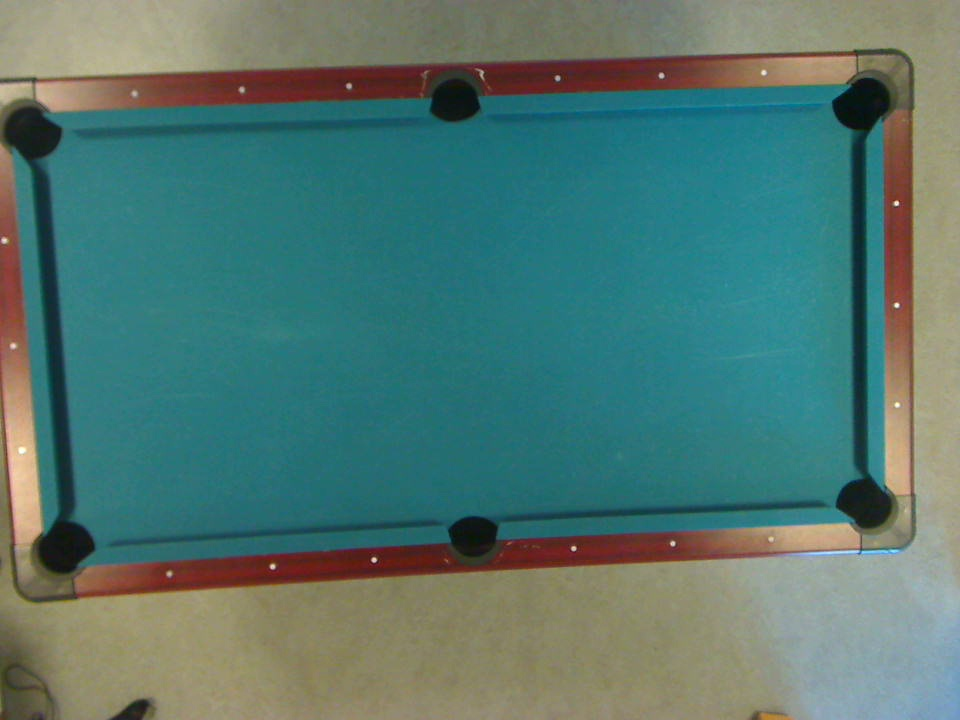
\includegraphics[width=0.4\textwidth]{images/test/light/input}
\end{center}
   \caption{The pool table used for testing.}
  \label{fig:pooltableimg}
\end{figure} 

The tests were made in two light conditions: normal and mixed. These conditions can be seen in figure \ref{fig:difflightcon}.

\begin{figure}[H]
  \centering
  \subfloat[Normal illumination]{\label{fig:gull}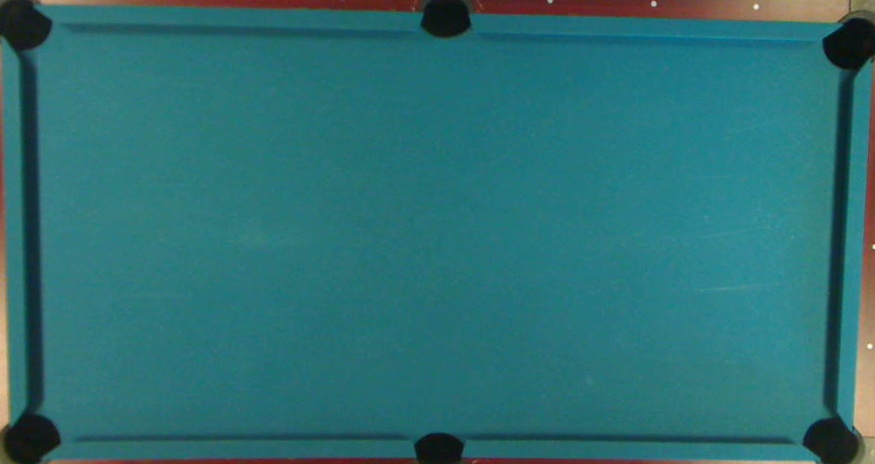
\includegraphics[width=0.48\textwidth]{images/test/light/detectedtable}}
  \quad           
  \subfloat[Mixed illumination]{\label{fig:tiger}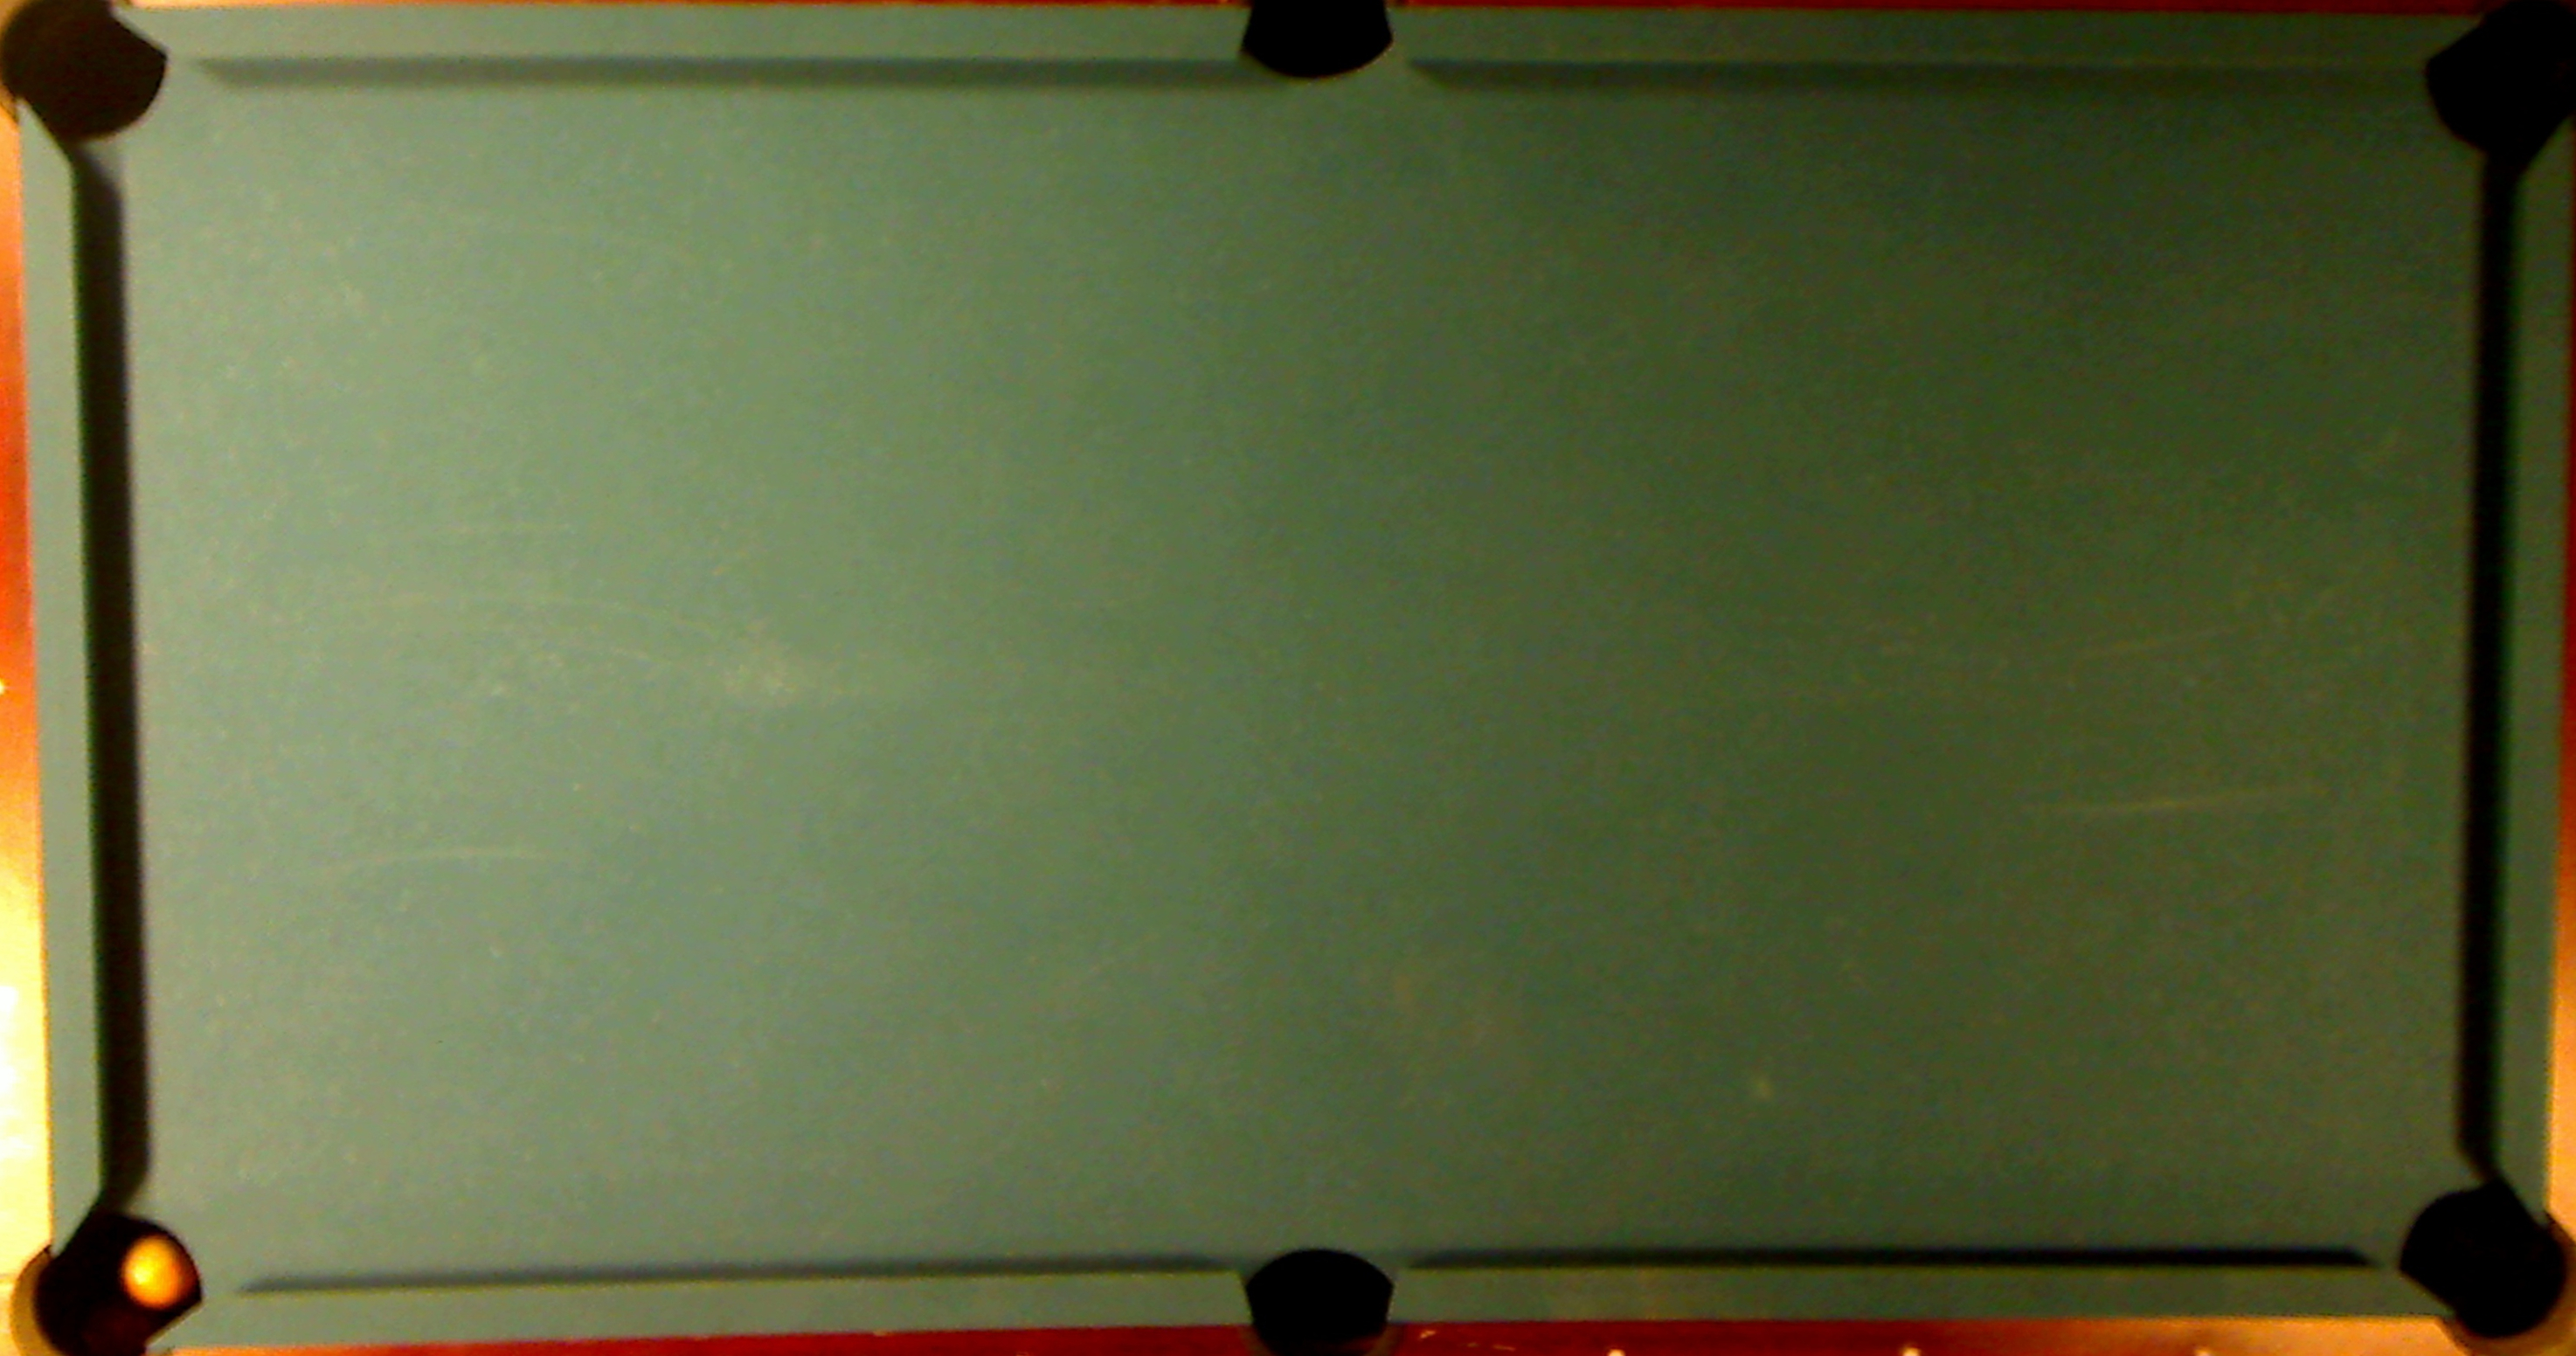
\includegraphics[width=0.48\textwidth]{images/test/mixed/detectedtable}}
   \caption{Table cloth in the two different light conditions.}
  \label{fig:difflightcon}
\end{figure}


\section{1) Detect position of table}

This was tested numerous times and if the position of the table is within the view of the camera the table will be found in both light conditions.

\section{2) Detect position of balls}
The precision of the ball positions is important, since the identification rests on having the correct positions. To test the detection, the balls have been positioned in different scenarios to test for different kinds of weaknesses in the detector. The following scenarios has been tested:
\begin{enumerate}
	\item Balls laying apart.
	\item Balls clustered by color
	\item Balls laying in start position as described in section \ref{sec:rules}.
\end{enumerate}
In some of the tests, two results have been recorded. One representing the best case scenario and one representing the worst case scenario. This is done to illustrate the differences observed during the test.

\subsection{Balls laying apart}
The least difficult test for the detection of balls is where the balls are laying apart. The result of the test with normal light can be seen in figure \ref{fig:apartnormal} and for the mixed light in figure \ref{fig:apartmixed}.

\begin{figure}[htpb]
  \centering
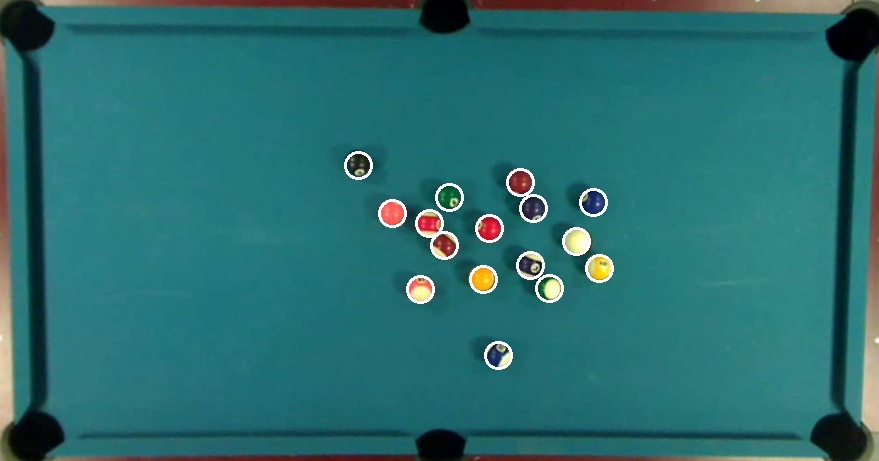
\includegraphics[width=0.5\textwidth]{images/test/light1/laying-apart}
   \caption{Balls laying apart - normal light.}
  \label{fig:apartnormal}
\end{figure}

\begin{figure}[htpb]
  \centering
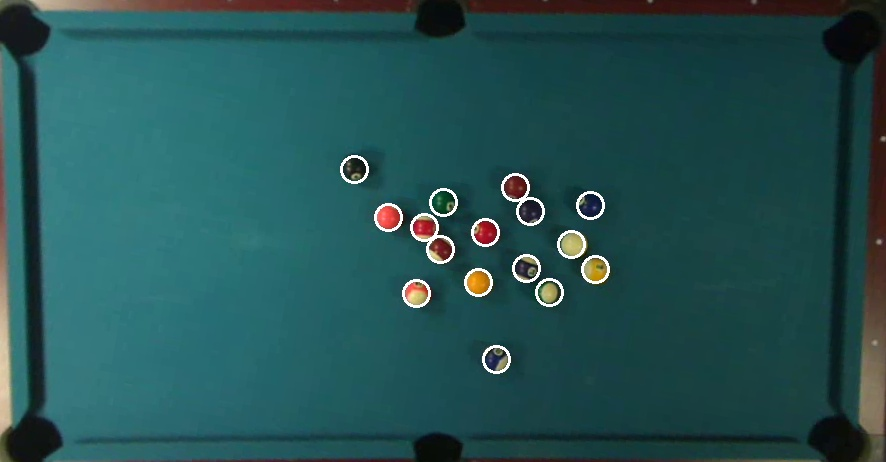
\includegraphics[width=0.5\textwidth]{images/test/mixed1/laying-apart}
   \caption{Balls laying apart - mixed light.}
  \label{fig:apartmixed}
\end{figure}

There is no significant change in the behavior of the system between the mixed, and the normal lighting. The balls are detected correctly in both the left and the right side of the table. This shows that the detection is adaptive towards change in lighting across the table in an uncluttered ball arrangement.

\subsection{Balls clustered by color}
As mentioned in section \ref{sec:balls-locate}, the ball detection works by finding areas that minimizes the color variance. To test for weaknesses in this method, the scenario seen in figures \ref{fig:clustersnormal} and \ref{fig:clustersmixed} is tested.
\begin{figure}[htpb]
  \centering
  \subfloat[Black ball low precision]{\label{fig:gull}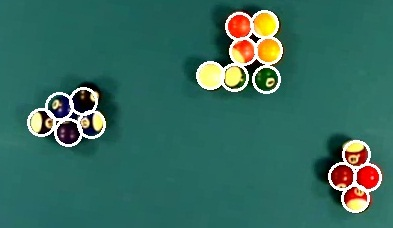
\includegraphics[width=0.4\textwidth]{images/test/light1/clusters-1}}
  \quad
   \subfloat[Two balls detected wrong]{\label{fig:tiger}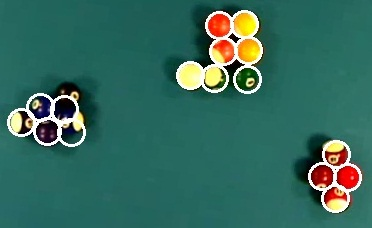
\includegraphics[width=0.4\textwidth]{images/test/light1/clusters-2}}
	\quad
   \caption{Balls in clusters - normal light.}
  \label{fig:clustersnormal}
\end{figure}

\begin{figure}[htpb]
  \centering
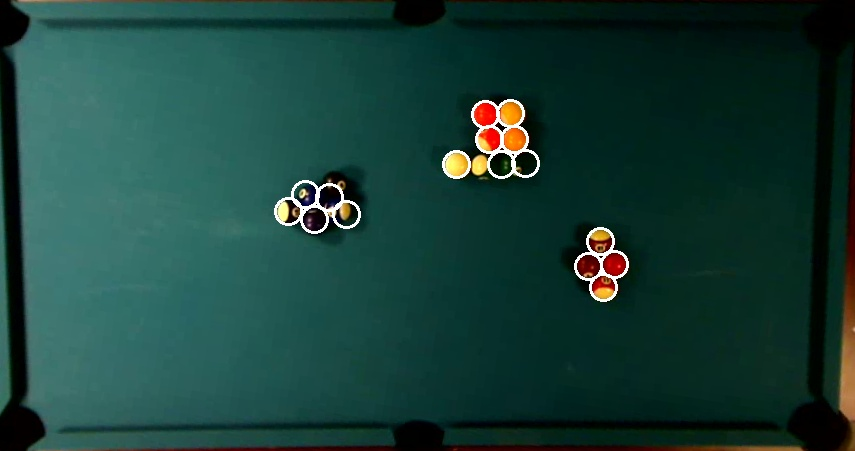
\includegraphics[width=0.5\textwidth]{images/test/mixed1/clusters-2}
   \caption{Balls in clusters - mixed light. Several detection problems.}
  \label{fig:clustersmixed}
\end{figure}
The balls are not correctly detected in this scenario. The problem is most significant in the left cluster that consists of the dark colored balls: purple, blue and black. The problem worsens when the image is darker in figure \ref{fig:clustersmixed}. The detection of the red colored balls does however not result in any errors or positional problems. 


\subsection{Balls laying in start position}
The balls are placed in the start position with all balls except the cue ball clustered. This is the most difficult condition to test positions of the pool balls. The test was done while the balls were laying still and the result of the test with normal light can be seen in figure \ref{fig:poolposstart} and for the mixed light in figure \ref{fig:poolposstart2}.

\begin{figure}[htpb]
  \centering
   \subfloat[Correct detection]{\label{fig:poolposstart-good}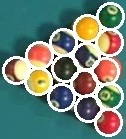
\includegraphics[width=0.2\textwidth]{images/test/light1/start-normal-1}}
\quad
   \subfloat[Incorrect detection]{\label{fig:poolposstart-bad}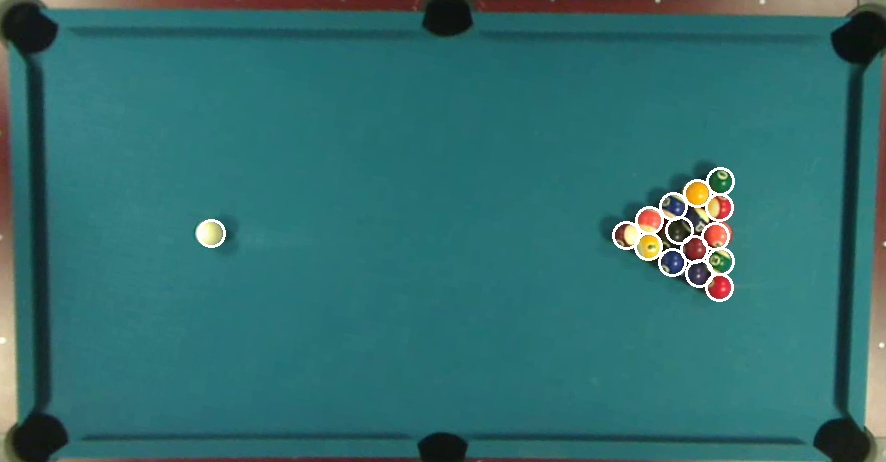
\includegraphics[width=0.2\textwidth]{images/test/light1/start-normal-2}}
   \caption{Balls in start position - normal light.}
  \label{fig:poolposstart}
\end{figure}

\begin{figure}[htpb]
  \centering
  \subfloat[Correct detection]{\label{fig:gull}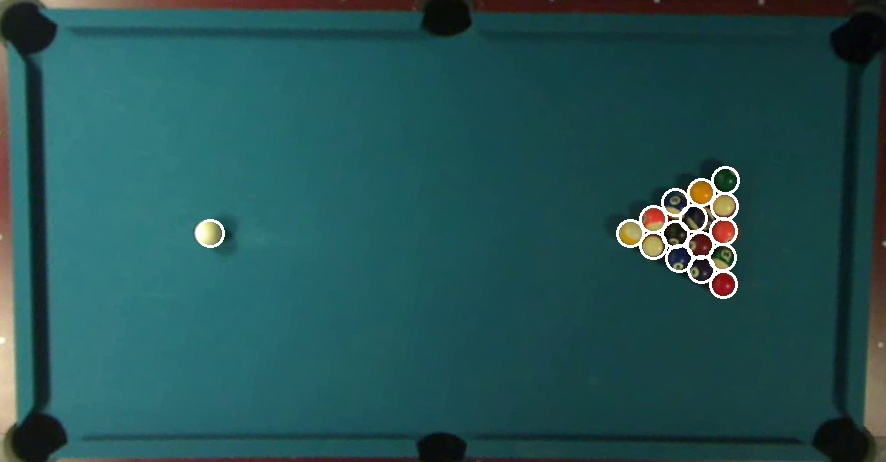
\includegraphics[width=0.2\textwidth]{images/test/mixed1/start-mixed-1}}
\quad
   \subfloat[Incorrect detection]{\label{fig:tiger}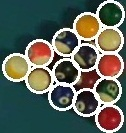
\includegraphics[width=0.2\textwidth]{images/test/mixed1/start-mixed-2}}
\quad
   \caption{Balls in start position - mixed light.}
  \label{fig:poolposstart2}
\end{figure}

The system performs almost equally in the light environment seen in figure \ref{fig:poolposstart} as in mixed lighting in figure \ref{fig:poolposstart2}. For the system to find all positions in this situation, it is important that the positions of the first detected balls are correct, because their positions will affect the rest of the detection as mentioned in section \ref{sec:balls-locate}. Problems arise in a situation like the one seen in figure \ref{fig:poolposstart-bad}. The black and orange balls have been inaccurately detected, and the consequence is that there is insufficient room to detect the striped purple 14.


\section{Identify balls with high accuracy}
The identification of the balls is done by first calibrating the system and then testing the identification with the balls facing in two different scenarios:

\begin{enumerate}
\setlength{\itemsep}{0mm}
	\item \textbf{Minimum} white area visible
	\item \textbf{Maximum} white area visible
\end{enumerate}
This is done to test the borderline cases for when a ball is considered solid, striped or white.

\subsection{Pool balls laying with minimum white facing up}
This scenario will test if the identifier has problems that causes striped balls to be identified as solid balls.
The result of the test with normal light can be seen in figure \ref{fig:minnormal} and for the mixed light in figure \ref{fig:minmixed}.
\begin{figure}[htpb]
  \centering
  \subfloat[Input image]{\label{fig:gull}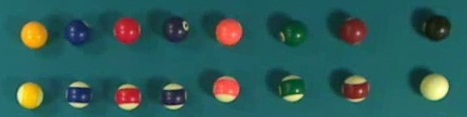
\includegraphics[width=0.5\textwidth]{images/test/light1/min-white-input}}
  \quad
   \subfloat[Found balls]{\label{fig:tiger}\includegraphics[width=0.5\textwidth]{images/test/light1/min-white-output}}
	\quad
   \caption{Balls having minimum white area visible - normal light.}
  \label{fig:minnormal}
\end{figure}

\begin{figure}[htpb]
  \centering
  \subfloat[Input image]{\label{fig:gull}\includegraphics[width=0.5\textwidth]{images/test/mixed1/min-white-input}}
  \quad
  \subfloat[Found balls]{\label{fig:tiger}\includegraphics[width=0.5\textwidth]{images/test/mixed1/min-white-output}}
  \quad
   \caption{Balls having minimum white area visible - mixed light.}
  \label{fig:minmixed}
\end{figure}
All balls on both mixed and normal lighting are correctly identified, except for striped brown 15 which has been classified as red striped 11. This occurs because of the colors begin close. None of the striped balls are misclassified as solids, independent of lighting conditions.

\subsection{Pool balls laying with maximum white facing up}
This test will illustrate if the ratio of white pixels is defined well enough to identify if the ball is solid or striped. Also the detection of correct colors will be tested. The result of the test with normal light can be seen in figure \ref{fig:maxnormal} and for the mixed light in figure \ref{fig:maxmixed}.

\begin{figure}[htpb]
  \centering
  \subfloat[Input image]{\label{fig:gull}\includegraphics[width=0.5\textwidth]{images/test/light1/max-white-input}}
  \quad
   \subfloat[Found balls]{\label{fig:tiger}\includegraphics[width=0.5\textwidth]{images/test/light1/max-white-output}}
	\quad
   \caption{Balls having maximum white area visible - normal light.}
  \label{fig:maxnormal}
\end{figure}

\begin{figure}[htpb]
  \centering
  \subfloat[Input image]{\label{fig:gull}\includegraphics[width=0.5\textwidth]{images/test/mixed1/max-white-input}}
  \quad
  \subfloat[Found balls]{\label{fig:tiger}\includegraphics[width=0.5\textwidth]{images/test/mixed1/max-white-output}}
  \quad
   \caption{Balls having maximum white area visible - mixed light.}
  \label{fig:maxmixed}
\end{figure}
The identification fails in both normal and mixed light. Identification of the striped balls in this scenario is problematic due to the small amount of color available. Most of the striped balls are however, identified as being striped in spite of the small amount of color. In the mixed light environment, several of the balls are identified as being the black 8-ball which is caused by the identifier being sensitive to the change in lighting.

\subsection{Position and identification of balls should be obtained within one second}
The system speed was tested with different sizes of video and image input from the used webcam. It will find the position and identify the balls within one second. This test was done on a Core-Duo L2400 running at 1.67 Ghz. 


	\section{System design and implementation}
		\label{sec:sysdesign}
		Small introduction.\\

\subsection{Program run flow}
The goal is to record a game of pool between every shots. To do this automatic, the program will have to know when a shot has been made and when to stop recording. The program flowchart can be seen in \ref{fig:program_flowchart}.\\

\begin{figure}[H]
\begin{center}
\leavevmode
\includegraphics[width=0.8\textwidth]{images/program_flowchart}
\end{center}
\caption{Flowchart of the PoolTracker program while running.}
\label{fig:program_flowchart}
\end{figure}

The game will start when the user decides to do so. The detection of occlusions will be explained in \ref{sec:shotdetection}. The movement of balls will be detected in\ref{sec:shotdetection} based on the balls positions which will be found in \ref{sec:balls-locate}.

\subsection{Calibration flow}
The calibration have to be done every time the camera changes position or when the system is installed for the first time. The calibration is done to locate table and to train the system with the colors of the balls. The calibration flowchart can be seen in \ref{fig:calib_flowchart}.\\

\begin{figure}[H]
\begin{center}
\leavevmode
\includegraphics[width=0.8\textwidth]{images/calib_flowchart}
\end{center}
\caption{Flowchart of the PoolTracker program in calibration.}
\label{fig:program_flowchart}
\end{figure}

Table location is explained in \ref{sec:table-locate}. The calibration of balls is explained in\ref{sec:ASKLDALD}.

\subsection{Code implementation}
The system is written in C\# using Microsoft Visual Studio 10. Since OpenCV\cite{opencv} is not compatible with C\# natively we use Emgu\cite{emgu} which is a wrapper for OpenCV to use in C\#. 

The design of the system has been done using UML diagrams. UML makes it easier knowing which parts communicated with other parts, their included methods and properties. The UML diagram for the PoolTracker can be seen in \ref{fig:uml}.

\begin{figure}[H]
\begin{center}
\leavevmode
\includegraphics[width=0.8\textwidth]{images/UML}
\end{center}
\caption{UML diagram of PoolTracker.}
\label{fig:uml}
\end{figure}


		
	\section{Locating table}
		\label{sec:table-intro}	
		Since the system does not know where the table is or which kind of table it is, a method for finding a general pool table have to be developed.The outcome of this section should be a method to determine where the playing field of the table is. This will serve as the ROI (region of interest) for further detection of balls. There are many methods that could be used to find the ROI. The key is to find a robust one that will also not be too computationally heavy. Besides finding the ROI, the angle of the table compared to the horizon must also be found. This will be used to rotate the input stream from the camera to 0\degree and later crop it to the ROI. The mask of the cloth will also be found for use in other parts of the system.\\
	
		
			\subsection{Locate table}
				\label{sec:table-locate}
				\subsection{Solutions Ideas:}

\begin{itemize}
\setlength{\itemsep}{0mm}
	\item Choose the ROI with user-input.
	\item Search for the table as the biggest contour.
	\item Searching for the pockets on the pool table.
	\item Finding the diamonds and using these to determine the ROI.
	\item Finding the most common colour (the cloth) and then find the outer points of the cloth.
\end{itemize}

\textbf{Choose The ROI With User-Input:}\\
This method would not require any image processing, but would require the user to set the ROI. This solution could be used if the chosen solution does not return a ROI due to difficult illumination or errors.

\textbf{Search For The Table As The Biggest Contour:}\\
The method was tried and gave mixed results. It was possible to segment the table using adaptive threshold and thereafter process it with OpenCV \cite{opencv} contour finding algorithm. This would find the outside of the table, but sometimes also the floor or anything underlying the table that was a bigger rectangle. \\

\textbf{Searching For The Pockets On The Pool Table:}\\
This proved to be easy to do by using the value part of the image in HSV colour space. Since the pockets are less illuminated than the rest of the table this should have a very low value. An example of this can be seen in\ref{fig:value_thres}. 

\begin{figure}[H]
\begin{center}
\leavevmode
\includegraphics[width=0.5\textwidth]{images/value_thres}
\end{center}
\caption{Value part of HSV image thresholded.}
\label{fig:value_thres}
\end{figure}

As seen in\ref{fig:value_thres} a leg is also selected as a part of the outcome of the threshold. Several tried showed that the method was not quite robust enough for further use.\\

\textbf{Finding The Diamonds and Use These To Determine The ROI:}\\
Much time was used with this approach. The idea was to find the diamonds and the use these to find the exact ROI. The specifications \ref{sec:rules} of a regulation size pool table states that a diamond has to be 93.5 mm from the nose of the cushion. By finding the length between each diamond, which was also strictly specified, it would be possible to find a pixel-to-meter ration and thereby finding the precise ROI.\\

Some progress was made, but eventually this method was abandoned due to the fact that many of the pool tables, including the one where pictures for this  project was taken, did not follow these regulations. The idea was also to use the distance between diamonds to determine the exact size of a ball. Another approach for this will have to be used.\\

\subsection{Chosen Solution:}

\textbf{Finding the most common colour (the cloth) and then find the outer points of the cloth.}\\
This solution showed to be the most robust since the cloth will take up at least 50\% and probably more of the entire image. This makes it a prime candidate for detecting. Also even in the odd coincidence where the colour of the floor and cloth are alike, the rails of the table will separate these and thereby still make it possible to detect the cloth.\\

As written in the pool table regulations \ref{sec:rules} the table has to be one of three colours: yellow-green, blue-green or electric blue. Different from the last method this seems to be the case for every pool table. That they have a solid colour which stands out.\\

This fact will be used as part of the solution for this problem. As shown on histograms in \ref{sec:analysisballstable} the hue part of the HSV colour space will to be good for separating the cloth from the rails and surroundings. Hue also has the useful property of, in theory, indifferent to illumination which should make it more robust for this solution. A flowchart of the solution can be seen in \ref{fig:tabledetect_flowchart}

%INDSÆT HISTOGRAM m. HUE over de fire forskellige billeder.

%The solution consists of the following steps:
%\begin{enumerate}
%\setlength{\itemsep}{0mm}
%	\item Convert the input image to HSV and make a new image for the hue.
%	\item Make a histogram of the value in the hue image.
%	\item Identify the pixels close to the maximum value of the hue histogram.
%	\item Remove noise by using a median filter.
%	\item Find the bounding box of the cloth and make a binary mask.
%	\item Find the angle of the cloth (and thereby table).
%	\item Output the ROI, angle and mask.
%\end{enumerate}

\begin{figure}[H]
\begin{center}
\leavevmode
\includegraphics[width=0.8\textwidth]{images/tabledetect_flowchart}
\end{center}
\caption{Flowchart of the chosen solution}
\label{fig:tabledetect_flowchart}
\end{figure}

\subsubsection{The Solution In Details:}
\textbf{1) Convert The Input Image to HSB and Make A New Image For The Hue:}\\
This is done using the build in functions of OpenCV\cite{opencv}\fxnote{Necessary to cite them every time?}.\\

\textbf{2) Making The Histogram:}\\
Using the class DenseHistogram in OpenCV\cite{opencv} the histogram is computed from the hue image. A range of 0-255 is chosen together with 255 bins.\\

\textbf{3) Identify The pixels close To The Maximum Value Of The Hue Histogram.}\\
After finding the bin with the maximum value an iteration of the whole image is done to identify pixels close to the maximum value. The pixels that lie close are set to 255 (white) and the others are set as 0 (black). A threshold of $\pm$ 20 is set based on different tries. Since the illumination of the cloth is not exactly the same this value have to be higher than first expected.\\

The image after the cloth identification can be seen in \ref{fig:aftercloth}.

\begin{figure}[H]
\begin{center}
\leavevmode
\includegraphics[width=0.5\textwidth]{images/aftercloth}
\end{center}
\caption{Image after cloth identification.}
\label{fig:aftercloth}
\end{figure}

\textbf{4) Remove Noise By Using A Median Filter:}\\
To remove noise from the image a median filter will be used. This allows the contour identifier in OpenCV\cite{opencv} to work optimal. If the median filter was not used potential contours could be much bigger than the cloth since one-pixel edges could connect across the rails from the cloth to floor. The outcome of the median filter can be seen in\ref{fig:afterclothmedian}

\begin{figure}[H]
\begin{center}
\leavevmode
\includegraphics[width=0.5\textwidth]{images/afterclothmedian}
\end{center}
\caption{Image after median filter, kernelsize = 3.}
\label{fig:afterclothmedian}
\end{figure}

\textbf{5) Find The Bounding Box Of The Cloth and Make A Binary Mask:}\\
The cloth now appears as the biggest BLOB in the image. To find the bounding box of the cloth OpenCVs \cite{opencv} FindContours function is used. It uses the metod Suzuki85 developed by S. Suzuki and K. Abe \cite{contour}. The code iterates through the different contours found by FindContours. These contours are tested whether they could be the cloth by using a few conditions:

\begin{itemize}
\setlength{\itemsep}{0mm}
	\item The table is, as written in the requirements specification \ref{sec:reqspec}, required to take up at least 75\% of the frame area. Since the rails of the table is not detected the condition is set to the contour area having to be at least 50\% of the frame area. 
	\item Since the FindContours function sometimes identifies the entire image as a contour, the detected contour have an area smaller than the area of the image.
\end{itemize}

All the found contours can be seen in \ref{fig:allcontours}.
\begin{figure}[H]
\begin{center}
\leavevmode
\includegraphics[width=0.5\textwidth]{images/allcontours}
\end{center}
\caption{All the contours found by FindContours after cloth identificationa and median filter.}
\label{fig:allcontours}
\end{figure}

The contour that is the output of the code above can be seen in \ref{fig:clothcontour}.
\begin{figure}[H]
\begin{center}
\leavevmode
\includegraphics[width=0.5\textwidth]{images/clothcontour}
\end{center}
\caption{Cloth contour found by FindContours after cloth identificationa and median filter.}
\label{fig:clothcontour}
\end{figure}

A mask of the found contours is made. Since the box of the contour has to have straight edges this will be used to remove rails and pockets that could be in the image so this is not used when having to find the balls.

\begin{figure}[H]
\centering
\subfloat[Mask of cloth and other contours.]
{
	\includegraphics[width=0.3\textwidth]{images/mask_1}
}
\subfloat[Found contour of cloth.]
{
	\includegraphics[width=0.3\textwidth]{images/mask_2}
}
\end{figure}

\textbf{6) Find The Angle Of The Cloth (And Thereby Table):}\\
To find the angle of the table the bounding rectangle of the contour of the cloth is divided into lines. A sort of the length is made and the longest line is selected. This line will always be the longest side of the table, the side that should be rotated to 0\degree. \\

The angle between the line and a horizontal line is calculated using the GetExteriorAngleDegree function in OpenCV\cite{opencv}. The angle found led to understand that there is a slight problem with the output as shown in \ref{fig:table_angle}.

\begin{figure}[H]
\begin{center}
\leavevmode
\includegraphics[width=0.5\textwidth]{images/table_angle}
\end{center}
\caption{The angle found between horizontal line and edge of table.}
\label{fig:table_angle}
\end{figure}

Therefore the if the angle is more than 90\degree is it calculated as angle = 180\degree-angle.\\

\textbf{7) Output The ROI, Angle and Mask:}\\
The angle and the box for the non-rotated image has been calculated. Since the calibration is not a time-critical part of the solution the ROI is found simply by rotating the image and running step 5 again.  This will rotate the image and then search for the ROI of the rotated image. A faster method would be calculating the new position of the ROI based on the rotated angle.
\\\\
The output can be seen in figure \ref{fig:tablelocateoutput}, with the original image, secondly the found ROI, thirdly the mask of the cloth and finally the output image.

\begin{figure}[H]
\centering
\subfloat[Input image.]
{
	\includegraphics[width=0.4\textwidth]{images/montage_input}
}
\subfloat[Cloth ROI.]
{
	\includegraphics[width=0.4\textwidth]{images/montage_contour}
}
\\
\subfloat[Mask of cloth.]
{
	\includegraphics[width=0.4\textwidth]{images/montage_mask}
}
\subfloat[The output after rotating, cropping and setting mask.]
{
	\includegraphics[width=0.4\textwidth]{images/montage_output}
}
\label{fig:tablelocateoutput}
\end{figure}

If the box for the non-rotated image is not found, then the angle is also not found. In this case the program will return a failure which indicates that the table is not found.
		
			%\subsection{Locate diamonds}
			%	\label{sec:table-diamonds}
			%	They are a few reasons for finding the diamonds and not only the outer or inner part of the table.

\begin{itemize}
	\item The diamonds provide key knowledge about pixel to meter ratio.
	\item To be able to have the smallest ROI to search for the balls. Note that the only fixed length to find the exact playing field are from the diamonds to the cushion as mentioned in \ref{sec:rules}
	\item For possible later implementation of UI where diamonds act as buttons.
\end{itemize}

The diamonds have several properties that will be used when locating them. As written in the pool table specifications \ref{sec:rules} the diamonds have a few useful properties:

\begin{itemize}
	\item They must be located with the same distance of each other.
	\item The center of each diamond must be located 93.5 mm from the nose of the cushion.
	\item They may be round or diamond-shaped.
	\item They stand out from their surroundings.
\end{itemize}

The table are be found in the previous section\ref{sec:table-locate} and thereby making the search-region for the diamonds smaller. Also, within the table there are very few contours that could appear to be a diamonds, where as outside the table the environment is completely different from place to place.\\

For robustly locating the diamonds the following approach has been used:
\begin{enumerate}
	\item Convert captured image to grayscale.
	\item Make binary with adaptive threshold.
	\item Find contours and sort them by size
	\item Do step 1 to 3 for several images.
	\item Find the contours that remain at same position throughout the sequence.
\end{enumerate}

%MAKE FLOWCHART.

\textbf{Convert to grayscale and use adaptive threshold:}\\
The captured image will be converted into grayscale for further process where it is made binary with adaptive threshold. This will provide much more invariance to light in the different regions of the table. More can be read about adaptive threshold in section \ref{sec:table-locate}.\\

%Insert Image

\textbf{Find contours:}\\
The next step is to find the contours in the binary image and sort them by size. The contours are found by using OpenCV build in contour detection algorithm \cite{contour}.

This will return a list of contours in the image\ref{fig:allcontours}.

\begin{figure}[H]
\begin{center}
\leavevmode
\includegraphics[width=0.5\textwidth]{images/allcontours.png}
\end{center}
\caption{All contours found in frame.}
\label{fig:allcontours}
\end{figure}

Many different contours are found as seen and therefore it is necessary to sort the contours based on their size and remove those that are outliers. A diamond should obey certain rules:

\begin{itemize}
	\item Size: The maximum diamond is [31.75 x 15.875 mm]. That is 0.0005 $m^2$. The smallest table is 3.5$m^2$. If the table completely fills up the frame the diamond can, at most, be $1/7000$ of the frame. By knowing the width and height of the image other contours above this size can be removed. Since the morphology operations changes the sizes the threshold is set at $1/3500$.
	\item The diamond is convex.
\end{itemize}

The area size used as reference is the median area of the list of contours. This should be approximately the area of a diamond. If the mean was used instead of the median a much larger value would be the reference, because of very big contours being found (in OpenCV implementation the image in itself is a contour).

The outcome is a list of possible diamonds.\\\\

\textbf{Find contours for a sequence of images:}\\
While testing, one of the major problems with finding the diamonds positions, was the noise introduced by various parameters (camera, lightning etc). The actual positions of the diamonds was found in every frame, but a lot of noise made found positions of diamonds elsewhere in the images. 
The noise changed from frame to frame.

Therefore, by using a sequence of images (video) and compare the positions found it is possible to eliminate the noise and only find the position of the diamonds.

Each time an image is processed the contours are saved in a list. When the decided number of images has been processed it is simply a process of comparing the lists and find the points that have not moved or at least have not moved very much.\\

\begin{figure}[H]
\begin{center}
\leavevmode
\includegraphics[width=0.5\textwidth]{images/image_seq_numbers.pdf}
\end{center}
\caption{Sequence of frames. The number of frames can be set as n.}
\label{fig:seq_img}
\end{figure}

\textbf{Find the contours that remain at same position throughout the sequence:}\\
A arbitrary point in the first frame is chosen. In all other frames the same position is searched for a contour. If this contour exists in every frame it is saved as a diamond. If it does not exist in every image it is not saved.

\begin{figure}[H]
\begin{center}
\leavevmode
\includegraphics[width=0.5\textwidth]{images/image_seq_pool.pdf}
\end{center}
\caption{Searching for a contour in from the first frame in all other frames.}
\label{fig:seq_img_pool}
\end{figure}


		
			%\subsection{Find size-references}
			%	\label{sec:table-sizes}
			%	The found points will be used to compute the size-references which will be used to know the size of a ball and also to find the playing surface ROI.




\textbf{Using the points to find the cloth:}
The reason for finding the diamonds is to be able to find the exact ROI to search for the balls. This ROI is defined as 93.5mm from the diamond in a orthogonal line to the edge of the cushion, as seen in \ref{fig:diamonddistance}.

\begin{figure}[H]
\begin{center}
\leavevmode
\includegraphics[width=0.5\textwidth]{images/diamonddistance.pdf }
\end{center}
\caption{Distance from diamond to nose of cushion.}
\label{fig:diamonddistance}
\end{figure}



	\section{Locating and identifying balls}
		\label{sec:balls-intro}	
		The main goal in this project is to detect and identify balls. There are different approaches to solving this problem, where some ideas concentrate on solving both problems at once by identifying balls directly and thereby also implicitly detecting them. Other solutions, like the one used in this project, does the detecting first to determine the regions of interest 	
		
			\subsection{Locate balls}
				\label{sec:balls-locate}
				The detection method can be divided into the following three steps:
\begin{enumerate}
  \item Preliminary segmentation
  \item Ball probability estimation
  \item Best candidates selection
\end{enumerate}

Preliminary segmentation is performed to decrease the ROI from the entire table area to areas that contains balls.

In step 2 the ROI is traversed, and a ball probability is computed at each possible ball location. 

To establish which of the positions inside the ROI are actual ball positions, the balls are selected from the list of probabilities starting with the most probable position.

\subsection{Preliminary Segmentation}
To decrease the ROI from the cloth area down to areas of the table that contains balls, a preliminary segmentation is performed. A color threshold on the hue image, removes all pixels that belong to the background leaving behind a mask that represents the balls.
\begin{figure}[htpb]
  \centering
  \subfloat[Original]{\label{fig:gull}\includegraphics[width=0.48\textwidth]{images/thres1before.jpg}}
  \quad           
  \subfloat[Segmentation]{\label{fig:tiger}\includegraphics[width=0.48\textwidth]{images/thres1after.jpg}}
   \caption{Color threshold to remove background}
  \label{fig:thres1}
\end{figure}
Figure \ref{fig:thres1} shows the result of the color threshold. In a situation like this where the balls are laying close to each other, the preliminary segmentation is not enough to successfully separate the balls. Balls in close proximity results in connected BLOBs after the threshold. These BLOBs could be separated using morphology operations but most of the information would be lost, causing the locations to lack precision. Instead of using the BLOBS directly, they are used as search regions for the balls.

\subsection{Ball Probability Estimation}
To be able to estimate the ball probability, we need to know the features that characterizes a ball. The following description can be formulated:
\begin{itemize}
\item The shape of the ball, in the image, is always a circle of fixed size
\item The color distribution consists of at least two of three parts:
	\begin{itemize}
		\item White
		\item Black (ball number)
		\item Primary ball color
	\end{itemize}
\end{itemize}
The black and cue balls has black and white, respectively, as their primary color, making them consist of only two distributions, whereas all other balls consists of three. This ball description allows us to formulate a measure for the probability that a given position in the image corresponds to the center of a ball.

If we ignore the black pixels from the ball number, the balls does only contain one primary color and white. A candidate ball position is defined as a circular ROI in the image having position the the center of the ROI circle.
The probability of a candidate position containing a ball can then be formulated as the ratio between the number of pixels in the ROI following this rule and the total pixels:
\begin{equation}
P_{ball}(x,y) = \frac{pixels_{primary} + pixels_{white}}{pixels_{total}}
\end{equation}
It is seen that the a region having only one color besides white maximizes the probability.
\begin{figure}[H]
\begin{center}
\includegraphics[width=0.6\textwidth]{images/ballfind.pdf}
\caption{The probability of a ball is evaluated in the image.}
\label{fig:ballfind}
\end{center}
\end{figure}
Figure \ref{fig:ballfind} shows the process of computing the ball probability. The probability is computed in every possible ball position.
A circular mask is placed in every position found by the preliminary segmentation. By using a circular mask, the system is able to get a better match against the circular ball regions. Inside the mask an HSB color histogram is computed. All pixels that have a hue value close to the background hue are ignored. The rest of the pixels are sorted into three categories: 
\begin{enumerate}
  \item White pixels
  \item Black pixels
  \item Colored pixels
\end{enumerate}
Pixels that have a saturation below a certain value are considered to be white. Pixels with brightness below a threshold are considered to be black. To make the system as color independent as possible, brightness is only used to identify black pixels. This is necessary because the black color is undefined in hue-saturation space. For further information see section \ref{sec:analballs} concerning analysis of ball color.

To determine the number of primary colored pixels, the variance of the colored pixels is analyzed. If the candidate position contains a ball, the distribution of the colored pixels is expected to be narrowly distributed around the mean of the ball color, like in figure \ref{fig:unimodal6}. If the position is between two or more balls the distribution will be multimodal and the variance higher like in figure \ref{fig:multimodal56}.

The pixels that are within a certain deviation of the mean hue are counted, resulting in a count of the number of primary colored pixels in the ball.

\begin{figure}[htpb]
  \centering
  \subfloat[Input]{\includegraphics[width=0.25\textwidth]{images/unimodal6-input}}
  \quad           
  \subfloat[Hue histogram]{\includegraphics[width=0.48\textwidth]{images/unimodal6}}
   \caption{Histogram of a correctly detected ball. Distribution is unimodal.}
  \label{fig:unimodal6}
\end{figure}
\begin{figure}[htpb]
  \centering
  \subfloat[Input]{\includegraphics[width=0.25\textwidth]{images/multimodal56-input}}
  \quad           
  \subfloat[Hue histogram]{\includegraphics[width=0.53\textwidth]{images/multimodal56}}
   \caption{Histogram of a bad detection. Distribution is multimodal.}
  \label{fig:multimodal56}
\end{figure}


If the number of black pixels is greater than the number of primary colored pixels, the number of black pixels is used as the number of primary pixels.
\subsection{Best Candidates Selection}
The result of the probability estimation is a sorted list of candidate positions, having the most probable position at the top of the list. The probability has been computed in every image position, which results in many overlapping positions. 

The final ball positions are found by traversing the list from the top and thus selecting the most probable positions first. A candidate will only be selected if there is not already a detected ball within one radius of the candidate position.  

The system continues to detect balls until 16 balls are found or the score is below a threshold. This threshold is set as a ratio of the total pixels in a ball. The whole process can be seen in figure \ref{fig:ballflowchart}.

\fxnote{Figure showing different distributions and their resulting ball probability}
\begin{figure}[htpb]
\begin{center}
\includegraphics[width=\textwidth]{images/ballflowchart.pdf}
\caption{Flowchart of the ball detection process.}
\label{fig:ballflowchart}
\end{center}
\end{figure}

A problem arises if a wrong match is found, which intersects candidates that have not yet been matched. The position of the intersected candidates will then be invalidated, because they are within the radius of a detected ball. It will then be impossible to find a new match in the region of the earlier wrong match. 
\begin{figure}[htpb]
\begin{center}
\includegraphics[width=0.3\textwidth]{images/wronglocate.jpg}
\caption{Consequence of wrong location detection. Red circles are ball detected balls}
\label{fig:wronglocate}
\end{center}
\end{figure}
Figure \ref{fig:wronglocate} shows the problem of a wrong match. The wrong match prevents several balls from being matched, and other balls from matching precisely.

\subsection{Detection Results}
Figure \ref{fig:detect} shows results of ball detection in 2 different situations. The detector shows good performance in uncluttered aswell as cluttered ball arrangements. The cluttered balls does however affect the precision of the detection

\begin{figure}[H]
  \centering
  \subfloat[No clutter]{\label{fig:gull}\includegraphics[width=0.4\textwidth]{images/detect1.jpg}}
  \quad           
  \subfloat[Clutter]{\label{fig:tiger}\includegraphics[width=0.4\textwidth]{images/detect2.jpg}}
   \caption{Results of ball detection. White circles indicate detected ball positions.}
  \label{fig:detect}
\end{figure}


		
			\subsection{Identifying balls}
				\label{sec:balls-id}
				Identification of the ball consists of two steps:
\begin{enumerate}
  \item Identifying the primary color of the ball
  \item Determining whether the ball is striped
\end{enumerate}
Both steps involves measuring the color distribution of the detected ball. The primary color in the distribution represents the color of the ball, while the amount of white in the distribution determines if the ball is striped.

\subparagraph{Vector Angle versus Euclidean Distance}
The color of a ball has to be classified to one of the eight different ball colors. This is achieved by calculating distances between the detected ball and model colors obtained from ball calibration. The detected ball is then classified as the model that has the shortest distance.

There are different ways of measuring difference between colors, and each of these measurements has their own advantages. In this section two methods for measuring color difference are compared to find the one most suitable for ball classification.
\fxnote{Figure describing angle vs. euclidean distance}
If we define two color vectors as $v_{1}$ and $v_{2}$, the euclidean distance between them is defined as
\begin{equation}
D_{E}(v_{1}, v_{2}) = ||v_{1}, v_{2}||
\end{equation}
where $||\bullet||$ is the $L_{2}$ vector norm. For the RGB coordinate system where $v = [r\;g\;b]^{T}$, the distance is calculated as
\begin{equation}
D_{E}(v_{1}, v_{2}) = \sqrt{(r_{1} - r_{2})^{2} + (r_{1} - r_{2})^{2} + (r_{1} - r_{2})^{2}}
\end{equation}
In RGB space the euclidean distance is more sensitive to differences in intensity than differences in color. This can cause problems if a light version of a color should match a darker version. Another measure, that does a better job of quantifying chromaticity difference in RGB space is the vector angle which is calculated as
\begin{equation}
cos \theta = \frac{v_{1}^ Tv_{2}}{||v_{1}|| ||v_{2}||}
\end{equation}
The vector angle between two colors having the same chromaticity but different intensity will be the same. \fxnote{as seen in figure} The vector angle in RGB is equivalent to using the hue distance in HSB\fxnote{I think it is}. Using the vector angle instead of converting the entire image to HSB can save computation time.\cite{angleVsEuclidean}

As written in section \ref{sec:analballs} regarding ball analysis, the balls should be separable in hue-saturation space, and thereby also separable by vector angle comparison. Experiments with both distances did however conclude that the angular distance between balls having similar hue was to short to give a robust classification. The vector angle, was for this reason abandoned, and the euclidean distance was used in the final implementation.

\paragraph{Color Comparison Strategy}\fxnote{Better name for paragraph?}
The ball color can be measured in two different ways: 
\begin{enumerate}
  \item Measure the distribution of the detected ball
  \item Use each pixel in the ball by itself
\end{enumerate}
The difference between the distribution of the detected ball and the model distributions can be measured using, e.g. Bhattacharyya or earth mover's distance. In this project, simpler metrics like the mean and the max has been used to compare ball distributions. 

Another way of looking at a ball is pixel by pixel. Each pixel is classified by itself, and the ball class is selected by taking the class where most of the ball pixels belong to. This is the approach used in this project. The thought behind this approach is that it will perform better against outliers and the varying number of colored pixels that is the nature of the pool balls. 

\paragraph{Implementation}
The classifier is trained by supervised training where the user selects the location for each of the solid colored balls. The mean RGB value is then extracted from each of the ball areas and this will serve as a model for color comparison. \fxnote{Figure showing sampling of color means from image during calibration}
The euclidean distance between al each pixel and the models are calculated to determine the ball that the pixel is most likely to represent.

\begin{table}[H]
\begin{center}
	\begin{tabular}{|l|c|c|c|c|c|c|c|c|c|}
		\hline
		Ball & c & \cellcolor{yellow}1 & \cellcolor{blue}2 & \cellcolor{red}3  & \cellcolor{purple}4 & \cellcolor{orange}5 & \cellcolor{green}6 & \cellcolor{brown}7 & \cellcolor{black}\textcolor{white}{8} \\
		\hline
		\includegraphics[]{images/ballsInVotes/0} & \cellcolor{gray}450 & 0 & 2 & 0 & 0 & 8 & 77 & 3 & 36\\
		\hline
		\includegraphics[]{images/ballsInVotes/1} & 5 & \cellcolor{gray}420 & 1 & 0 & 1 & 15 & 64 & 35 & 35\\
		\hline
		\includegraphics[]{images/ballsInVotes/2} & 15 & 0 & \cellcolor{gray}437 & 0 & 37 & 6 & 32 & 0 & 49\\
		\hline
		\includegraphics[]{images/ballsInVotes/3} & 11 & 0 & 20 & \cellcolor{gray}333 & 34 & 51 & 12 & 113 & 2\\
		\hline
		\includegraphics[]{images/ballsInVotes/4} & 19 & 0 & 87 & 0 & \cellcolor{gray}293 & 8 & 24 & 3 & 142\\
		\hline
		\includegraphics[]{images/ballsInVotes/5} & 2 & 0 & 16 & 27 & 12 & \cellcolor{gray}452 & 23 & 34 & 10\\
		\hline
		\includegraphics[]{images/ballsInVotes/6} & 35 & 0 & 9 & 0 & 0 & 3 & \cellcolor{gray}504 & 1 & 24\\
		\hline
		\includegraphics[]{images/ballsInVotes/7} & 0 & 0 & 18 & 13 & 54 & 18 & 14 & \cellcolor{gray}413 & 46\\
		\hline
		\includegraphics[]{images/ballsInVotes/8} & 21 & 0 & 27 & 0 & 33 & 12 & 74 & 12 & \cellcolor{gray}397\\
		\hline
		\includegraphics[]{images/ballsInVotes/9} & \cellcolor{gray}170 & \cellcolor{gray}291 & 0 & 0 & 0 & 3 & 74 & 18 & 20\\
		\hline
		\includegraphics[]{images/ballsInVotes/10} & \cellcolor{gray}145 & 1 & \cellcolor{gray}232 & 0 & 40 & 16 & 66 & 9 & 67\\
		\hline
		\includegraphics[]{images/ballsInVotes/11} & \cellcolor{gray}94 & 3 & 5 & \cellcolor{gray}229 & 7 & 109 & 30 & 65 & 34\\
		\hline
		\includegraphics[]{images/ballsInVotes/12} & \cellcolor{gray}142 & 0 & 6 & 0 & 106 & 21 & 82 & 25 & \cellcolor{red}194\\
		\hline
		\includegraphics[]{images/ballsInVotes/13} & \cellcolor{gray}256 & 2 & 7 & 2 & 23 & \cellcolor{gray}177 & 37 & 54 & 18 \\
		\hline
		\includegraphics[]{images/ballsInVotes/14} & \cellcolor{gray}253 & 0 & 9 & 0 & 1 & 6 & \cellcolor{gray}202 & 3 & 102\\
		\hline
		\includegraphics[]{images/ballsInVotes/15} & \cellcolor{gray}107 & 0 & 7 & 14 & 19 & 47 & 49 & \cellcolor{gray}311 & 22\\
		\hline
	\end{tabular}
\end{center}
	\label{table:ballvote}
	\caption{Detected balls and their votes. Gray shading marks a correct identification.}
\end{table}
Table \ref{table:ballvote} shows the votes for the detected balls in a session where all 16 balls were present on the table. Each of the balls are identified by the maximum number of votes for a color, indicated by a gray background for a correct match, and red for incorrect match. Balls having white votes above a certain threshold are classified as striped balls, indicated by a gray background in both their primary color and cue.

In the situation seen in table \ref{table:ballvote} the only error comes from the striped purple 14 being identified as the black. The same problem is spotted in the solid variant: the purple 6, which also has a high number of black votes. The solid balls has more colored pixels to represent the color, making the problem worst among striped balls.

\chapter{System test}
	\label{sec:system-test}
	To understand if the solution works it will be subjected to a test with origin in the requirement specification in section \ref{sec:reqspec}. The requirements, which will be tested, are listed here:

\begin{enumerate}
\setlength{\itemsep}{0mm}
	\item Detect position of table.
	\item Detect position of balls.
	\item Identify balls with high accuracy.
	\item Position and identification of balls should be obtained within one second
	\item Work with mixed light conditions and not only those stated in WPAB rules \ref{sec:rules}.
\end{enumerate}

The tests for the first four requirements will be done individually with the different lighting as described in section \ref{sec:testsetup}. The fifth requirement will be tested within the other requirements by altering the light.

\section{Test setup}
\label{sec:testsetup}
The test were conducted in the multimedia lab located in room A6-314 on Niels Jernes Vej 12 in Aalborg where image and video material for the solution to this project were made. 

%A second smaller test, to illustrate that the solution will work for different pool tables, is conducted in the DE-Klub which is a student bar located in A4-101 at Frederik Bajers Vej 7 in Aalborg. 
The pool table can be seen in figure \ref{fig:pooltableimg}. The videos used for the test can be found on the CD-Rom enclosed with this report.

\begin{figure}[H]
\begin{center}
\leavevmode
\includegraphics[width=0.4\textwidth]{images/test/light/input}
\end{center}
   \caption{The pool table used for testing.}
  \label{fig:pooltableimg}
\end{figure} 

The tests were made in two light conditions: normal and mixed. These conditions can be seen in figure \ref{fig:difflightcon}.

\begin{figure}[H]
  \centering
  \subfloat[Normal illumination]{\label{fig:gull}\includegraphics[width=0.48\textwidth]{images/test/light/detectedtable}}
  \quad           
  \subfloat[Mixed illumination]{\label{fig:tiger}\includegraphics[width=0.48\textwidth]{images/test/mixed/detectedtable}}
   \caption{Table cloth in the two different light conditions.}
  \label{fig:difflightcon}
\end{figure}


\section{1) Detect position of table}

This was tested numerous times and if the position of the table is within the view of the camera the table will be found in both light conditions.

\section{2) Detect position of balls}
The precision of the ball positions is important, since the identification rests on having the correct positions. To test the detection, the balls have been positioned in different scenarios to test for different kinds of weaknesses in the detector. The following scenarios has been tested:
\begin{enumerate}
	\item Balls laying apart.
	\item Balls clustered by color
	\item Balls laying in start position as described in section \ref{sec:rules}.
\end{enumerate}
In some of the tests, two results have been recorded. One representing the best case scenario and one representing the worst case scenario. This is done to illustrate the differences observed during the test.

\subsection{Balls laying apart}
The least difficult test for the detection of balls is where the balls are laying apart. The result of the test with normal light can be seen in figure \ref{fig:apartnormal} and for the mixed light in figure \ref{fig:apartmixed}.

\begin{figure}[htpb]
  \centering
\includegraphics[width=0.5\textwidth]{images/test/light1/laying-apart}
   \caption{Balls laying apart - normal light.}
  \label{fig:apartnormal}
\end{figure}

\begin{figure}[htpb]
  \centering
\includegraphics[width=0.5\textwidth]{images/test/mixed1/laying-apart}
   \caption{Balls laying apart - mixed light.}
  \label{fig:apartmixed}
\end{figure}

There is no significant change in the behavior of the system between the mixed, and the normal lighting. The balls are detected correctly in both the left and the right side of the table. This shows that the detection is adaptive towards change in lighting across the table in an uncluttered ball arrangement.

\subsection{Balls clustered by color}
As mentioned in section \ref{sec:balls-locate}, the ball detection works by finding areas that minimizes the color variance. To test for weaknesses in this method, the scenario seen in figures \ref{fig:clustersnormal} and \ref{fig:clustersmixed} is tested.
\begin{figure}[htpb]
  \centering
  \subfloat[Black ball low precision]{\label{fig:gull}\includegraphics[width=0.4\textwidth]{images/test/light1/clusters-1}}
  \quad
   \subfloat[Two balls detected wrong]{\label{fig:tiger}\includegraphics[width=0.4\textwidth]{images/test/light1/clusters-2}}
	\quad
   \caption{Balls in clusters - normal light.}
  \label{fig:clustersnormal}
\end{figure}

\begin{figure}[htpb]
  \centering
\includegraphics[width=0.5\textwidth]{images/test/mixed1/clusters-2}
   \caption{Balls in clusters - mixed light. Several detection problems.}
  \label{fig:clustersmixed}
\end{figure}
The balls are not correctly detected in this scenario. The problem is most significant in the left cluster that consists of the dark colored balls: purple, blue and black. The problem worsens when the image is darker in figure \ref{fig:clustersmixed}. The detection of the red colored balls does however not result in any errors or positional problems. 


\subsection{Balls laying in start position}
The balls are placed in the start position with all balls except the cue ball clustered. This is the most difficult condition to test positions of the pool balls. The test was done while the balls were laying still and the result of the test with normal light can be seen in figure \ref{fig:poolposstart} and for the mixed light in figure \ref{fig:poolposstart2}.

\begin{figure}[htpb]
  \centering
   \subfloat[Correct detection]{\label{fig:poolposstart-good}\includegraphics[width=0.2\textwidth]{images/test/light1/start-normal-1}}
\quad
   \subfloat[Incorrect detection]{\label{fig:poolposstart-bad}\includegraphics[width=0.2\textwidth]{images/test/light1/start-normal-2}}
   \caption{Balls in start position - normal light.}
  \label{fig:poolposstart}
\end{figure}

\begin{figure}[htpb]
  \centering
  \subfloat[Correct detection]{\label{fig:gull}\includegraphics[width=0.2\textwidth]{images/test/mixed1/start-mixed-1}}
\quad
   \subfloat[Incorrect detection]{\label{fig:tiger}\includegraphics[width=0.2\textwidth]{images/test/mixed1/start-mixed-2}}
\quad
   \caption{Balls in start position - mixed light.}
  \label{fig:poolposstart2}
\end{figure}

The system performs almost equally in the light environment seen in figure \ref{fig:poolposstart} as in mixed lighting in figure \ref{fig:poolposstart2}. For the system to find all positions in this situation, it is important that the positions of the first detected balls are correct, because their positions will affect the rest of the detection as mentioned in section \ref{sec:balls-locate}. Problems arise in a situation like the one seen in figure \ref{fig:poolposstart-bad}. The black and orange balls have been inaccurately detected, and the consequence is that there is insufficient room to detect the striped purple 14.


\section{Identify balls with high accuracy}
The identification of the balls is done by first calibrating the system and then testing the identification with the balls facing in two different scenarios:

\begin{enumerate}
\setlength{\itemsep}{0mm}
	\item \textbf{Minimum} white area visible
	\item \textbf{Maximum} white area visible
\end{enumerate}
This is done to test the borderline cases for when a ball is considered solid, striped or white.

\subsection{Pool balls laying with minimum white facing up}
This scenario will test if the identifier has problems that causes striped balls to be identified as solid balls.
The result of the test with normal light can be seen in figure \ref{fig:minnormal} and for the mixed light in figure \ref{fig:minmixed}.
\begin{figure}[htpb]
  \centering
  \subfloat[Input image]{\label{fig:gull}\includegraphics[width=0.5\textwidth]{images/test/light1/min-white-input}}
  \quad
   \subfloat[Found balls]{\label{fig:tiger}\includegraphics[width=0.5\textwidth]{images/test/light1/min-white-output}}
	\quad
   \caption{Balls having minimum white area visible - normal light.}
  \label{fig:minnormal}
\end{figure}

\begin{figure}[htpb]
  \centering
  \subfloat[Input image]{\label{fig:gull}\includegraphics[width=0.5\textwidth]{images/test/mixed1/min-white-input}}
  \quad
  \subfloat[Found balls]{\label{fig:tiger}\includegraphics[width=0.5\textwidth]{images/test/mixed1/min-white-output}}
  \quad
   \caption{Balls having minimum white area visible - mixed light.}
  \label{fig:minmixed}
\end{figure}
All balls on both mixed and normal lighting are correctly identified, except for striped brown 15 which has been classified as red striped 11. This occurs because of the colors begin close. None of the striped balls are misclassified as solids, independent of lighting conditions.

\subsection{Pool balls laying with maximum white facing up}
This test will illustrate if the ratio of white pixels is defined well enough to identify if the ball is solid or striped. Also the detection of correct colors will be tested. The result of the test with normal light can be seen in figure \ref{fig:maxnormal} and for the mixed light in figure \ref{fig:maxmixed}.

\begin{figure}[htpb]
  \centering
  \subfloat[Input image]{\label{fig:gull}\includegraphics[width=0.5\textwidth]{images/test/light1/max-white-input}}
  \quad
   \subfloat[Found balls]{\label{fig:tiger}\includegraphics[width=0.5\textwidth]{images/test/light1/max-white-output}}
	\quad
   \caption{Balls having maximum white area visible - normal light.}
  \label{fig:maxnormal}
\end{figure}

\begin{figure}[htpb]
  \centering
  \subfloat[Input image]{\label{fig:gull}\includegraphics[width=0.5\textwidth]{images/test/mixed1/max-white-input}}
  \quad
  \subfloat[Found balls]{\label{fig:tiger}\includegraphics[width=0.5\textwidth]{images/test/mixed1/max-white-output}}
  \quad
   \caption{Balls having maximum white area visible - mixed light.}
  \label{fig:maxmixed}
\end{figure}
The identification fails in both normal and mixed light. Identification of the striped balls in this scenario is problematic due to the small amount of color available. Most of the striped balls are however, identified as being striped in spite of the small amount of color. In the mixed light environment, several of the balls are identified as being the black 8-ball which is caused by the identifier being sensitive to the change in lighting.

\subsection{Position and identification of balls should be obtained within one second}
The system speed was tested with different sizes of video and image input from the used webcam. It will find the position and identify the balls within one second. This test was done on a Core-Duo L2400 running at 1.67 Ghz. 

	
\chapter{Conclusion}
	\label{sec:conclusion}
	To understand if the solution works it will be subjected to a test with origin in the requirement specification in section \ref{sec:reqspec}. The requirements, which will be tested, are listed here:

\begin{enumerate}
\setlength{\itemsep}{0mm}
	\item Detect position of table.
	\item Detect position of balls.
	\item Identify balls with high accuracy.
	\item Position and identification of balls should be obtained within one second
	\item Work with mixed light conditions and not only those stated in WPAB rules \ref{sec:rules}.
\end{enumerate}

The tests for the first four requirements will be done individually with the different lighting as described in section \ref{sec:testsetup}. The fifth requirement will be tested within the other requirements by altering the light.

\section{Test setup}
\label{sec:testsetup}
The test were conducted in the multimedia lab located in room A6-314 on Niels Jernes Vej 12 in Aalborg where image and video material for the solution to this project were made. 

%A second smaller test, to illustrate that the solution will work for different pool tables, is conducted in the DE-Klub which is a student bar located in A4-101 at Frederik Bajers Vej 7 in Aalborg. 
The pool table can be seen in figure \ref{fig:pooltableimg}. The videos used for the test can be found on the CD-Rom enclosed with this report.

\begin{figure}[H]
\begin{center}
\leavevmode
\includegraphics[width=0.4\textwidth]{images/test/light/input}
\end{center}
   \caption{The pool table used for testing.}
  \label{fig:pooltableimg}
\end{figure} 

The tests were made in two light conditions: normal and mixed. These conditions can be seen in figure \ref{fig:difflightcon}.

\begin{figure}[H]
  \centering
  \subfloat[Normal illumination]{\label{fig:gull}\includegraphics[width=0.48\textwidth]{images/test/light/detectedtable}}
  \quad           
  \subfloat[Mixed illumination]{\label{fig:tiger}\includegraphics[width=0.48\textwidth]{images/test/mixed/detectedtable}}
   \caption{Table cloth in the two different light conditions.}
  \label{fig:difflightcon}
\end{figure}


\section{1) Detect position of table}

This was tested numerous times and if the position of the table is within the view of the camera the table will be found in both light conditions.

\section{2) Detect position of balls}
The precision of the ball positions is important, since the identification rests on having the correct positions. To test the detection, the balls have been positioned in different scenarios to test for different kinds of weaknesses in the detector. The following scenarios has been tested:
\begin{enumerate}
	\item Balls laying apart.
	\item Balls clustered by color
	\item Balls laying in start position as described in section \ref{sec:rules}.
\end{enumerate}
In some of the tests, two results have been recorded. One representing the best case scenario and one representing the worst case scenario. This is done to illustrate the differences observed during the test.

\subsection{Balls laying apart}
The least difficult test for the detection of balls is where the balls are laying apart. The result of the test with normal light can be seen in figure \ref{fig:apartnormal} and for the mixed light in figure \ref{fig:apartmixed}.

\begin{figure}[htpb]
  \centering
\includegraphics[width=0.5\textwidth]{images/test/light1/laying-apart}
   \caption{Balls laying apart - normal light.}
  \label{fig:apartnormal}
\end{figure}

\begin{figure}[htpb]
  \centering
\includegraphics[width=0.5\textwidth]{images/test/mixed1/laying-apart}
   \caption{Balls laying apart - mixed light.}
  \label{fig:apartmixed}
\end{figure}

There is no significant change in the behavior of the system between the mixed, and the normal lighting. The balls are detected correctly in both the left and the right side of the table. This shows that the detection is adaptive towards change in lighting across the table in an uncluttered ball arrangement.

\subsection{Balls clustered by color}
As mentioned in section \ref{sec:balls-locate}, the ball detection works by finding areas that minimizes the color variance. To test for weaknesses in this method, the scenario seen in figures \ref{fig:clustersnormal} and \ref{fig:clustersmixed} is tested.
\begin{figure}[htpb]
  \centering
  \subfloat[Black ball low precision]{\label{fig:gull}\includegraphics[width=0.4\textwidth]{images/test/light1/clusters-1}}
  \quad
   \subfloat[Two balls detected wrong]{\label{fig:tiger}\includegraphics[width=0.4\textwidth]{images/test/light1/clusters-2}}
	\quad
   \caption{Balls in clusters - normal light.}
  \label{fig:clustersnormal}
\end{figure}

\begin{figure}[htpb]
  \centering
\includegraphics[width=0.5\textwidth]{images/test/mixed1/clusters-2}
   \caption{Balls in clusters - mixed light. Several detection problems.}
  \label{fig:clustersmixed}
\end{figure}
The balls are not correctly detected in this scenario. The problem is most significant in the left cluster that consists of the dark colored balls: purple, blue and black. The problem worsens when the image is darker in figure \ref{fig:clustersmixed}. The detection of the red colored balls does however not result in any errors or positional problems. 


\subsection{Balls laying in start position}
The balls are placed in the start position with all balls except the cue ball clustered. This is the most difficult condition to test positions of the pool balls. The test was done while the balls were laying still and the result of the test with normal light can be seen in figure \ref{fig:poolposstart} and for the mixed light in figure \ref{fig:poolposstart2}.

\begin{figure}[htpb]
  \centering
   \subfloat[Correct detection]{\label{fig:poolposstart-good}\includegraphics[width=0.2\textwidth]{images/test/light1/start-normal-1}}
\quad
   \subfloat[Incorrect detection]{\label{fig:poolposstart-bad}\includegraphics[width=0.2\textwidth]{images/test/light1/start-normal-2}}
   \caption{Balls in start position - normal light.}
  \label{fig:poolposstart}
\end{figure}

\begin{figure}[htpb]
  \centering
  \subfloat[Correct detection]{\label{fig:gull}\includegraphics[width=0.2\textwidth]{images/test/mixed1/start-mixed-1}}
\quad
   \subfloat[Incorrect detection]{\label{fig:tiger}\includegraphics[width=0.2\textwidth]{images/test/mixed1/start-mixed-2}}
\quad
   \caption{Balls in start position - mixed light.}
  \label{fig:poolposstart2}
\end{figure}

The system performs almost equally in the light environment seen in figure \ref{fig:poolposstart} as in mixed lighting in figure \ref{fig:poolposstart2}. For the system to find all positions in this situation, it is important that the positions of the first detected balls are correct, because their positions will affect the rest of the detection as mentioned in section \ref{sec:balls-locate}. Problems arise in a situation like the one seen in figure \ref{fig:poolposstart-bad}. The black and orange balls have been inaccurately detected, and the consequence is that there is insufficient room to detect the striped purple 14.


\section{Identify balls with high accuracy}
The identification of the balls is done by first calibrating the system and then testing the identification with the balls facing in two different scenarios:

\begin{enumerate}
\setlength{\itemsep}{0mm}
	\item \textbf{Minimum} white area visible
	\item \textbf{Maximum} white area visible
\end{enumerate}
This is done to test the borderline cases for when a ball is considered solid, striped or white.

\subsection{Pool balls laying with minimum white facing up}
This scenario will test if the identifier has problems that causes striped balls to be identified as solid balls.
The result of the test with normal light can be seen in figure \ref{fig:minnormal} and for the mixed light in figure \ref{fig:minmixed}.
\begin{figure}[htpb]
  \centering
  \subfloat[Input image]{\label{fig:gull}\includegraphics[width=0.5\textwidth]{images/test/light1/min-white-input}}
  \quad
   \subfloat[Found balls]{\label{fig:tiger}\includegraphics[width=0.5\textwidth]{images/test/light1/min-white-output}}
	\quad
   \caption{Balls having minimum white area visible - normal light.}
  \label{fig:minnormal}
\end{figure}

\begin{figure}[htpb]
  \centering
  \subfloat[Input image]{\label{fig:gull}\includegraphics[width=0.5\textwidth]{images/test/mixed1/min-white-input}}
  \quad
  \subfloat[Found balls]{\label{fig:tiger}\includegraphics[width=0.5\textwidth]{images/test/mixed1/min-white-output}}
  \quad
   \caption{Balls having minimum white area visible - mixed light.}
  \label{fig:minmixed}
\end{figure}
All balls on both mixed and normal lighting are correctly identified, except for striped brown 15 which has been classified as red striped 11. This occurs because of the colors begin close. None of the striped balls are misclassified as solids, independent of lighting conditions.

\subsection{Pool balls laying with maximum white facing up}
This test will illustrate if the ratio of white pixels is defined well enough to identify if the ball is solid or striped. Also the detection of correct colors will be tested. The result of the test with normal light can be seen in figure \ref{fig:maxnormal} and for the mixed light in figure \ref{fig:maxmixed}.

\begin{figure}[htpb]
  \centering
  \subfloat[Input image]{\label{fig:gull}\includegraphics[width=0.5\textwidth]{images/test/light1/max-white-input}}
  \quad
   \subfloat[Found balls]{\label{fig:tiger}\includegraphics[width=0.5\textwidth]{images/test/light1/max-white-output}}
	\quad
   \caption{Balls having maximum white area visible - normal light.}
  \label{fig:maxnormal}
\end{figure}

\begin{figure}[htpb]
  \centering
  \subfloat[Input image]{\label{fig:gull}\includegraphics[width=0.5\textwidth]{images/test/mixed1/max-white-input}}
  \quad
  \subfloat[Found balls]{\label{fig:tiger}\includegraphics[width=0.5\textwidth]{images/test/mixed1/max-white-output}}
  \quad
   \caption{Balls having maximum white area visible - mixed light.}
  \label{fig:maxmixed}
\end{figure}
The identification fails in both normal and mixed light. Identification of the striped balls in this scenario is problematic due to the small amount of color available. Most of the striped balls are however, identified as being striped in spite of the small amount of color. In the mixed light environment, several of the balls are identified as being the black 8-ball which is caused by the identifier being sensitive to the change in lighting.

\subsection{Position and identification of balls should be obtained within one second}
The system speed was tested with different sizes of video and image input from the used webcam. It will find the position and identify the balls within one second. This test was done on a Core-Duo L2400 running at 1.67 Ghz. 

	
\chapter{Future work}
	\label{sec:futurework}
	To understand if the solution works it will be subjected to a test with origin in the requirement specification in section \ref{sec:reqspec}. The requirements, which will be tested, are listed here:

\begin{enumerate}
\setlength{\itemsep}{0mm}
	\item Detect position of table.
	\item Detect position of balls.
	\item Identify balls with high accuracy.
	\item Position and identification of balls should be obtained within one second
	\item Work with mixed light conditions and not only those stated in WPAB rules \ref{sec:rules}.
\end{enumerate}

The tests for the first four requirements will be done individually with the different lighting as described in section \ref{sec:testsetup}. The fifth requirement will be tested within the other requirements by altering the light.

\section{Test setup}
\label{sec:testsetup}
The test were conducted in the multimedia lab located in room A6-314 on Niels Jernes Vej 12 in Aalborg where image and video material for the solution to this project were made. 

%A second smaller test, to illustrate that the solution will work for different pool tables, is conducted in the DE-Klub which is a student bar located in A4-101 at Frederik Bajers Vej 7 in Aalborg. 
The pool table can be seen in figure \ref{fig:pooltableimg}. The videos used for the test can be found on the CD-Rom enclosed with this report.

\begin{figure}[H]
\begin{center}
\leavevmode
\includegraphics[width=0.4\textwidth]{images/test/light/input}
\end{center}
   \caption{The pool table used for testing.}
  \label{fig:pooltableimg}
\end{figure} 

The tests were made in two light conditions: normal and mixed. These conditions can be seen in figure \ref{fig:difflightcon}.

\begin{figure}[H]
  \centering
  \subfloat[Normal illumination]{\label{fig:gull}\includegraphics[width=0.48\textwidth]{images/test/light/detectedtable}}
  \quad           
  \subfloat[Mixed illumination]{\label{fig:tiger}\includegraphics[width=0.48\textwidth]{images/test/mixed/detectedtable}}
   \caption{Table cloth in the two different light conditions.}
  \label{fig:difflightcon}
\end{figure}


\section{1) Detect position of table}

This was tested numerous times and if the position of the table is within the view of the camera the table will be found in both light conditions.

\section{2) Detect position of balls}
The precision of the ball positions is important, since the identification rests on having the correct positions. To test the detection, the balls have been positioned in different scenarios to test for different kinds of weaknesses in the detector. The following scenarios has been tested:
\begin{enumerate}
	\item Balls laying apart.
	\item Balls clustered by color
	\item Balls laying in start position as described in section \ref{sec:rules}.
\end{enumerate}
In some of the tests, two results have been recorded. One representing the best case scenario and one representing the worst case scenario. This is done to illustrate the differences observed during the test.

\subsection{Balls laying apart}
The least difficult test for the detection of balls is where the balls are laying apart. The result of the test with normal light can be seen in figure \ref{fig:apartnormal} and for the mixed light in figure \ref{fig:apartmixed}.

\begin{figure}[htpb]
  \centering
\includegraphics[width=0.5\textwidth]{images/test/light1/laying-apart}
   \caption{Balls laying apart - normal light.}
  \label{fig:apartnormal}
\end{figure}

\begin{figure}[htpb]
  \centering
\includegraphics[width=0.5\textwidth]{images/test/mixed1/laying-apart}
   \caption{Balls laying apart - mixed light.}
  \label{fig:apartmixed}
\end{figure}

There is no significant change in the behavior of the system between the mixed, and the normal lighting. The balls are detected correctly in both the left and the right side of the table. This shows that the detection is adaptive towards change in lighting across the table in an uncluttered ball arrangement.

\subsection{Balls clustered by color}
As mentioned in section \ref{sec:balls-locate}, the ball detection works by finding areas that minimizes the color variance. To test for weaknesses in this method, the scenario seen in figures \ref{fig:clustersnormal} and \ref{fig:clustersmixed} is tested.
\begin{figure}[htpb]
  \centering
  \subfloat[Black ball low precision]{\label{fig:gull}\includegraphics[width=0.4\textwidth]{images/test/light1/clusters-1}}
  \quad
   \subfloat[Two balls detected wrong]{\label{fig:tiger}\includegraphics[width=0.4\textwidth]{images/test/light1/clusters-2}}
	\quad
   \caption{Balls in clusters - normal light.}
  \label{fig:clustersnormal}
\end{figure}

\begin{figure}[htpb]
  \centering
\includegraphics[width=0.5\textwidth]{images/test/mixed1/clusters-2}
   \caption{Balls in clusters - mixed light. Several detection problems.}
  \label{fig:clustersmixed}
\end{figure}
The balls are not correctly detected in this scenario. The problem is most significant in the left cluster that consists of the dark colored balls: purple, blue and black. The problem worsens when the image is darker in figure \ref{fig:clustersmixed}. The detection of the red colored balls does however not result in any errors or positional problems. 


\subsection{Balls laying in start position}
The balls are placed in the start position with all balls except the cue ball clustered. This is the most difficult condition to test positions of the pool balls. The test was done while the balls were laying still and the result of the test with normal light can be seen in figure \ref{fig:poolposstart} and for the mixed light in figure \ref{fig:poolposstart2}.

\begin{figure}[htpb]
  \centering
   \subfloat[Correct detection]{\label{fig:poolposstart-good}\includegraphics[width=0.2\textwidth]{images/test/light1/start-normal-1}}
\quad
   \subfloat[Incorrect detection]{\label{fig:poolposstart-bad}\includegraphics[width=0.2\textwidth]{images/test/light1/start-normal-2}}
   \caption{Balls in start position - normal light.}
  \label{fig:poolposstart}
\end{figure}

\begin{figure}[htpb]
  \centering
  \subfloat[Correct detection]{\label{fig:gull}\includegraphics[width=0.2\textwidth]{images/test/mixed1/start-mixed-1}}
\quad
   \subfloat[Incorrect detection]{\label{fig:tiger}\includegraphics[width=0.2\textwidth]{images/test/mixed1/start-mixed-2}}
\quad
   \caption{Balls in start position - mixed light.}
  \label{fig:poolposstart2}
\end{figure}

The system performs almost equally in the light environment seen in figure \ref{fig:poolposstart} as in mixed lighting in figure \ref{fig:poolposstart2}. For the system to find all positions in this situation, it is important that the positions of the first detected balls are correct, because their positions will affect the rest of the detection as mentioned in section \ref{sec:balls-locate}. Problems arise in a situation like the one seen in figure \ref{fig:poolposstart-bad}. The black and orange balls have been inaccurately detected, and the consequence is that there is insufficient room to detect the striped purple 14.


\section{Identify balls with high accuracy}
The identification of the balls is done by first calibrating the system and then testing the identification with the balls facing in two different scenarios:

\begin{enumerate}
\setlength{\itemsep}{0mm}
	\item \textbf{Minimum} white area visible
	\item \textbf{Maximum} white area visible
\end{enumerate}
This is done to test the borderline cases for when a ball is considered solid, striped or white.

\subsection{Pool balls laying with minimum white facing up}
This scenario will test if the identifier has problems that causes striped balls to be identified as solid balls.
The result of the test with normal light can be seen in figure \ref{fig:minnormal} and for the mixed light in figure \ref{fig:minmixed}.
\begin{figure}[htpb]
  \centering
  \subfloat[Input image]{\label{fig:gull}\includegraphics[width=0.5\textwidth]{images/test/light1/min-white-input}}
  \quad
   \subfloat[Found balls]{\label{fig:tiger}\includegraphics[width=0.5\textwidth]{images/test/light1/min-white-output}}
	\quad
   \caption{Balls having minimum white area visible - normal light.}
  \label{fig:minnormal}
\end{figure}

\begin{figure}[htpb]
  \centering
  \subfloat[Input image]{\label{fig:gull}\includegraphics[width=0.5\textwidth]{images/test/mixed1/min-white-input}}
  \quad
  \subfloat[Found balls]{\label{fig:tiger}\includegraphics[width=0.5\textwidth]{images/test/mixed1/min-white-output}}
  \quad
   \caption{Balls having minimum white area visible - mixed light.}
  \label{fig:minmixed}
\end{figure}
All balls on both mixed and normal lighting are correctly identified, except for striped brown 15 which has been classified as red striped 11. This occurs because of the colors begin close. None of the striped balls are misclassified as solids, independent of lighting conditions.

\subsection{Pool balls laying with maximum white facing up}
This test will illustrate if the ratio of white pixels is defined well enough to identify if the ball is solid or striped. Also the detection of correct colors will be tested. The result of the test with normal light can be seen in figure \ref{fig:maxnormal} and for the mixed light in figure \ref{fig:maxmixed}.

\begin{figure}[htpb]
  \centering
  \subfloat[Input image]{\label{fig:gull}\includegraphics[width=0.5\textwidth]{images/test/light1/max-white-input}}
  \quad
   \subfloat[Found balls]{\label{fig:tiger}\includegraphics[width=0.5\textwidth]{images/test/light1/max-white-output}}
	\quad
   \caption{Balls having maximum white area visible - normal light.}
  \label{fig:maxnormal}
\end{figure}

\begin{figure}[htpb]
  \centering
  \subfloat[Input image]{\label{fig:gull}\includegraphics[width=0.5\textwidth]{images/test/mixed1/max-white-input}}
  \quad
  \subfloat[Found balls]{\label{fig:tiger}\includegraphics[width=0.5\textwidth]{images/test/mixed1/max-white-output}}
  \quad
   \caption{Balls having maximum white area visible - mixed light.}
  \label{fig:maxmixed}
\end{figure}
The identification fails in both normal and mixed light. Identification of the striped balls in this scenario is problematic due to the small amount of color available. Most of the striped balls are however, identified as being striped in spite of the small amount of color. In the mixed light environment, several of the balls are identified as being the black 8-ball which is caused by the identifier being sensitive to the change in lighting.

\subsection{Position and identification of balls should be obtained within one second}
The system speed was tested with different sizes of video and image input from the used webcam. It will find the position and identify the balls within one second. This test was done on a Core-Duo L2400 running at 1.67 Ghz. 


\bibliography{kilder}

\end{document}
